    \documentclass{diploma}
    \usepackage{cmap} % for serchable pdf's
    \usepackage[T2A]{fontenc} 
    \usepackage[utf8]{inputenc}
    \usepackage[english,russian]{babel}
    \usepackage{indentfirst}
    \usepackage[colorlinks=true,urlcolor=black,linkcolor=black,filecolor=black,citecolor=black,unicode,pdftex]{hyperref}
    \usepackage{graphicx}
    \usepackage{caption}
    \usepackage{pdfpages}
    \usepackage{amsmath}
    \usepackage{dot2texi}
    \usepackage{tikz}
    \usetikzlibrary{shapes,arrows}
    \usepackage{listings}
%\usepackage[titletoc]{appendix} 
%\usepackage{citehack}
\renewcommand{\baselinestretch}{1.5}


% to economize paper (for printing) uncomment next 5 lines
%\textwidth=190mm
%\textheight=250mm
%\topmargin=-20mm
%\oddsidemargin=-15mm
%\evensidemargin=-15mm



\begin{document}
\sloppy

\title{Генератор синтаксических анализаторов для неоднозначных контекстно-свободных грамматик}
\author{Григорьева Семёна Вячеславовича}
\university{Санкт-Петербургский Государственный Университет}
\facility{Математико-механический факультет}
\group{461}
\position{студента}
\chair{Кафедра системного программирования}
\leaderPosition{к.ф.-м.н.}
\leader{А.С. Лукичев}
\criticPosition{д.ф.-м.н., проф.}
\critic{Б.К. Мартыненко}
\chairLeaderPosition{д.ф.-м.н., проф.}
\chairLeader{А.Н. Терехов }
\city{Санкт-Петербург}
\yr{2010}

\maketitle
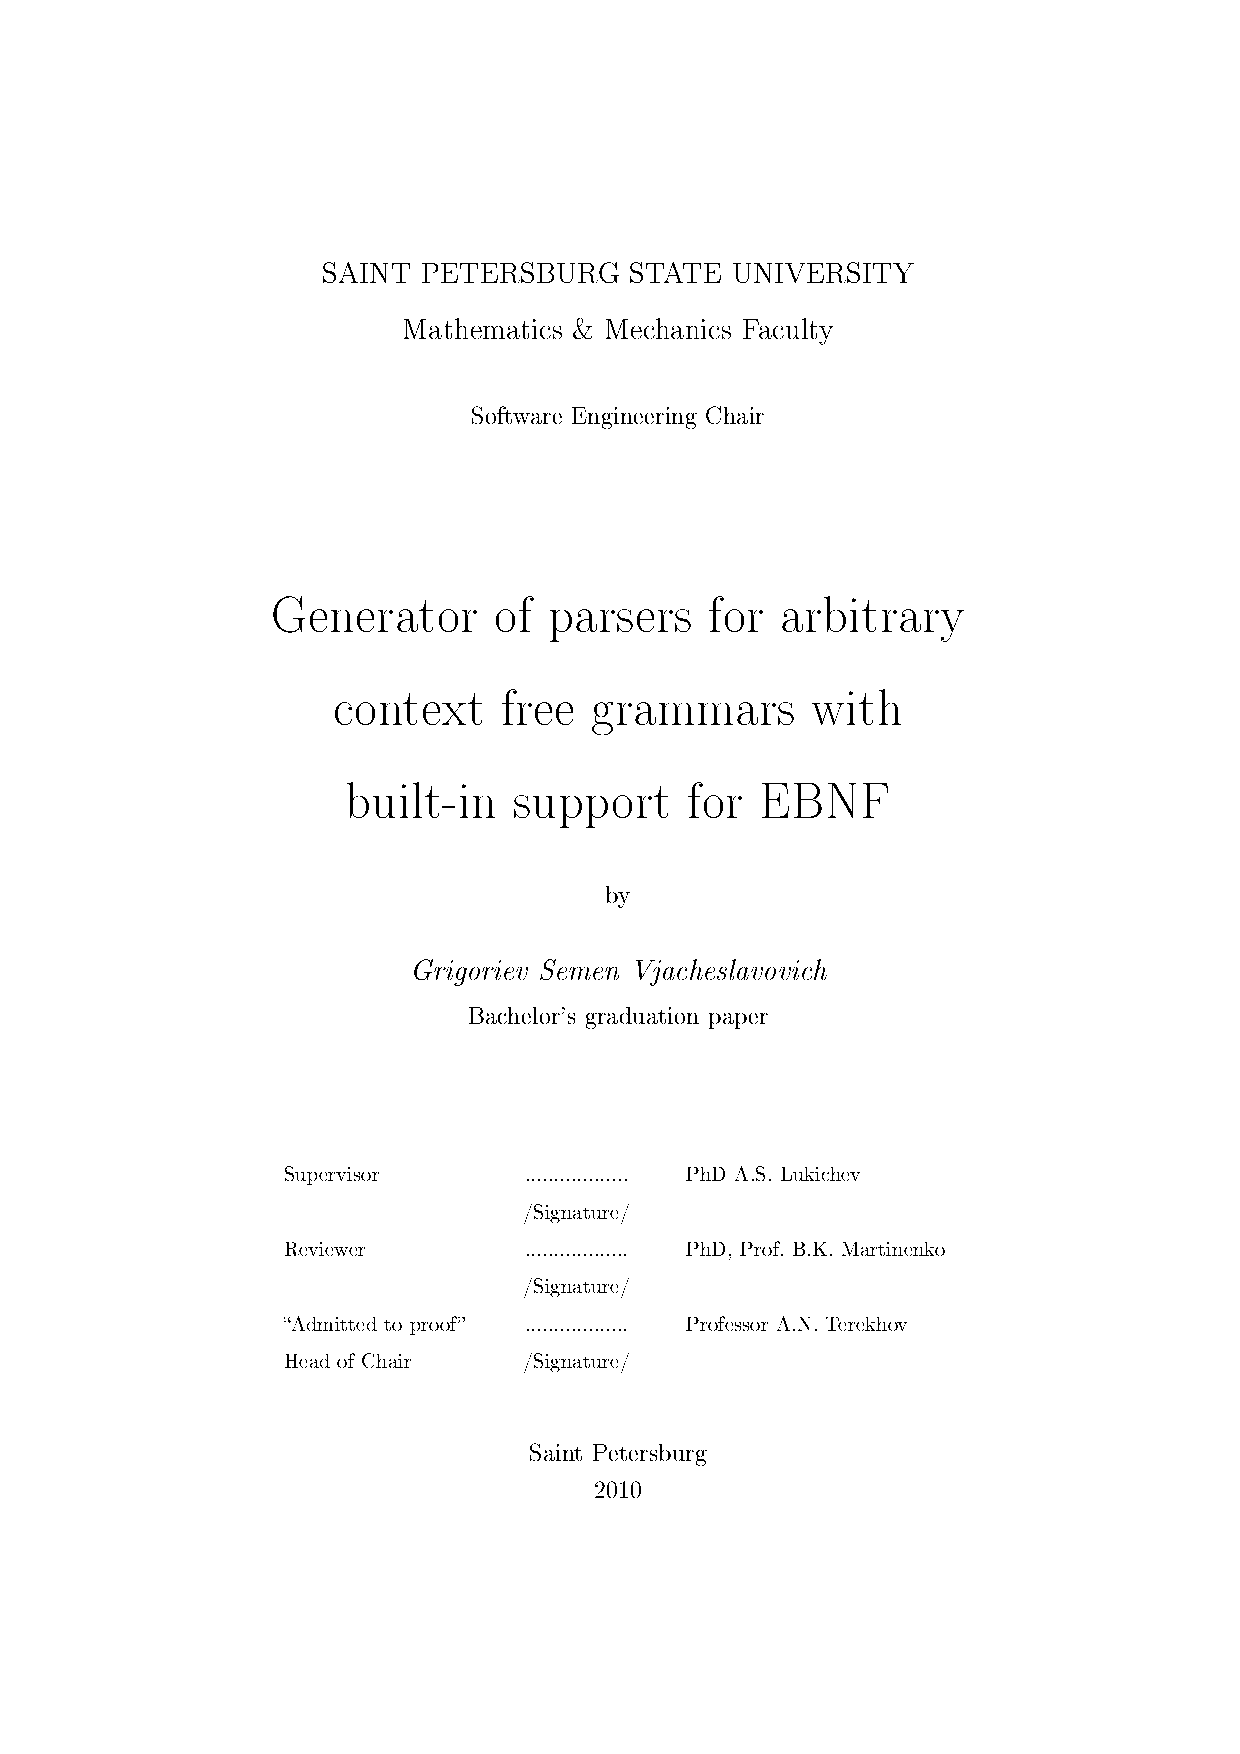
\includepdf{SemenDiplomaTitle_en.pdf}
\setcounter{page}{2}
\tableofcontents
\newpage


\section{Введение}	

Задачи автоматизированного  реинжиниринга  программ~\cite{Reeng} выдвигают особые требования~\cite{CurrentParsTechn} к генераторам синтаксических анализаторов. Во многом это связано с тем, что теория синтаксически управляемой трансляции развивалась одновременно языками, сейчас называемых устаревшими (legacy languages). Тогда еще не были получены основные теоретические результаты, положенные в основу наиболее распространенных современных генераторов синтаксических анализаторов. Поэтому устаревшие языки имеют особенности, затрудняющие синтаксический анализ даже с использованием современных инструментов (например ASF+SDF~\cite{ASF+SDF}, Elkhound~\cite{Elkhound}), которые значительно упрощают создание анализаторов.

Для устаревшего языка сложно (а зачастую и невозможно) задать однозначную контекстно-свободную грамматику. Необходимо существенно преобразовать его спецификацию, которая приводится в документации, чтобы получить такую грамматику. Но после этого она серьёзно усложняется и на её сопровождение требуется больше ресурсов~\cite{CurrentParsTechn}. Поэтому устаревший язык обычно задается с помощью неоднозначной контекстно-свободной грамматики.

При решении задач реинжиниринга часто требуются преобразования уже существующей грамматики. С одной стороны, при разработке  грамматики могут быть допущены неточности, с другой, документация устаревших языков и, в особенности, их диалектов может содержать ошибки, быть неполной или вообще отсутствовать. В результате, в целевом инструменте появляются ошибки, многие из которых возможно выявить только на этапе его тестирования. Для их исправления необходимо корректировать исходную грамматику. При этом, зачастую, изменение одного правила приводит к появлению десятков конфликтов в грамматике~\cite{CurrentParsTechn}, которые необходимо разрешать "`вручную"', что требует большого количества времени.

Кроме этого, на практике часто оказывается удобным иметь описание нескольким диалектов одного языка в одной грамматике. Это позволяет переиспользовать общие части грамматики, так как диалекты, как правило, имеют много общего. В то же время диалекты имеют характерные синтаксические конструкции, которые позволят автоматически определять принадлежность входной строки тому или иному диалекту. Однако при таких описаниях часто возникают конфликты, которые так же приходится разрешать "`вручную"'.

Для решения этих задач предлагается использовать неоднозначные контекстно-свободные грамматики и соответствующие инструменты построения анализаторов~\cite{CurrentParsTechn}. Основная особенность этих инструментов -- алгоритм, который способен работать с неоднозначными грамматиками (GLR-алгоритм). Анализатор, построенный по неоднозначной  грамматике с помощью данного алгоритма, в общем случае, в результате разбора строит не единственное дерево, а несколько деревьев -- лес, содержащий все возможные варианты вывода. Дальнейшая работа с полученным лесом организуется исходя из требований и  особенностей решаемой задачи. Это избавляет он необходимости "`ручного"' устранения конфликтов, что существенно сокращает время и упрощает разработку грамматики. Важным плюсом является ещё и то, что код становится более компактным и сопровождаемым.
      
%который можно сократить, используя специальные фильтры, а можно ,при задании в одной спецификации нескольких диалектов, вернуть весь лес для дальнейшего выбора нужного дерева/диалекта.   

%Работу GLR-алгоритма  можно рассматривать как параллельное исполнение набора LR-анализаторов. При этом данный набор дополняется процедурой управления стеками, оптимизирующей представление стеков путем их «склеивания» и «расклеивания», что позволяет хранить и строить параллельные выводы в рамках одного LR-анализатора, лишь в моменты их различия добавляя параллельный анализатор.

%Оказалось, что весьма наглядно такой алгоритм может быть представлен в виде набора взаимно-рекурсивных функций ~\cite{Non-det-rec-asc},~\cite{RECURSIVE-ASCENT PARSING},~\cite{RecursiveAscentParsing}. При этом расклеивание стека получается естественным образом как ветвление в одной из функций, а обратное склеивание может быть реализовано как кэширование результата функции.

Стоит отметить, что по производительности такой анализатор, являясь некоторой "`надстройкой"' \ над LR-анализатором, незначительно ему уступает. На сегодняшний день в соотношении производительность/класс разбираемых языков GLR-алгоритм выглядит наиболее предпочтительно.

Удобным способом определения грамматики языка программирования является расширенная форма Бэкуса-Наура(EBNF)~\cite{ISOEBNF} -- правила в такой грамматике в правых частях содержат регулярные выражения. На практике, использование EBNF позволяет упростить и сократить описание языка, сделать его более понятным. Кроме того, документация по языку, как правило, содержит конструкции EBNF. Однако многие современные инструменты не поддерживают EBNF-конструкции.

При работе с инструментом пользователь ожидает получить результат, описанный в терминах заданной им грамматики. Это выдвигает дополнительные требования к алгоритму. В случае, если входная грамматика была каким-либо образом преобразована, например с целью раскрыть конструкции EBNF, то появляется необходимость в построении "`обратного"' \ преобразования. Это преобразование должно "`перевести"' \ результат обратно в термины входной грамматики. Такие преобразования  требуют дополнительных ресурсов и усложняют инструмент. Поэтому наиболее предпочтительными является алгоритмы, работающие без дополнительных преобразований грамматики.

В рамках данной работы ставится цель разработки прототипа генератора анализаторов, позволяющего работать с неоднозначными расширенными контекстно-свободными грамматиками, предоставляющего, в то же время, ставшие привычными средства реализации трансляции, такие как атрибуты.

\clearpage
\section{���������� ������}

� ������ ������ ���� ���������� ��������� ������:
\begin{itemize}
	\item ������� ����������-����������� ��������;
	\item ������� ����������� ����������-����������� ��������� ��� ������ � EBNF ������������;
	\item ������� ����������� ������ ���������� ��������� ��� ������ � ������������ ������������� ����������-���������� ������������;
	\item ����������� �������� ���������� �������������� ������������, ���������� �� ����������-���������� ��������� � ������������ ����������� ������� ��������� �����:
		\begin{itemize}
		  \item ������ � �������������� �� ������������
			\item ������ � ������������ �� ������������ ��� �� ��������������
			\item ������ s-����������� ������������
		\end{itemize}
\end{itemize}
\clearpage
\section{Основные определения}

Определим ряд понятий и введём некоторые обозначения, необходимых для дальнейшего изложения.
\\
\\
	{\bfseries Определение 1.} \textit{Конструкции регулярнх выражений}: будем говорить, что грамматика (правило) содержит конструкции регулярных выражений, если в записи правых частей правил используются элементы синтаксиса регулярных выражений (альтернатива, замыкание).
\\
	{\bfseries Определение 2.} \textit{Раскрытие конструкций регулярных выражений}: будем называть раскрытием конструкций регулярных выражений такое преобразование грамматики (правила), при котором исходная грамматика заменяется на эквивалентную, не содержащую конструкций регулярных выражений.
\\
	{\bfseries Определение 3.} \textit{Дерево вывода строки в EBNF-грамматике}: упорядоченное помеченное дерево $D$ называется деревом вывода в EBNF-грамматике $G(S)=(N,T,P,S)$, если выполнены следующие условия:

\begin{enumerate}
	\item корень дерева $D$ помечен $S$;
	\item каждый лист помечен либо $a \in T$, либо $\varepsilon$;
	\item каждая внутренняя вершина помечена нетерминалом;
	\item если $N$ -- нетерминал, которым помечена внутренняя вершина и $X_1,...,X_n$ - метки ее прямых потомков в указанном порядке, то существует правило $N \rightarrow Y_1...Y_n \in P$ такое, что строка $X_1...X_n$ пораждается регулярным выражением $Y_1...Y_n$.
\end{enumerate}
	{\bfseries Определение 4.} \textit{Непосредственная поддержка EBNF-грамматик}: будем говорить, что инструмент непосредственно поддерживает EBNF-грамматики, если он работает с ними без раскрытия конструкций регулярных выражений.
\\
 	{\bfseries Определение 5.} \textit{Побочный эффект}: будем говорить, что функция или атрибут обладают побочным эффектом, если в процессе их вычислений возможно читать и модифицировать значения глобальных переменных, осуществлять операции ввода/вывода, реагировать на исключительные ситуации, вызывать их обработчики.



Для примеров псевдокода, приводимых далее, будем использовать синтаксические соглашения, принятые в языке программирования F\#.

%\begin{itemize}

	%\item GLR: Generalized LR Parsing~\cite{CurrentParsTechn}

	%%\item ДКА: детерминированный конечный автомат. Такой автомат, в котором для каждой последовательности входных символов существует лишь одно состояние, в которое автомат может перейти из текущего~\cite{DrgBook}.
	
	%%\item НКА: недетерминированный конечный автомат~\cite{DrgBook}.
	
	%\item Замыкание: q* = q$ \bigcup \{B\rightarrow.c | A \rightarrow a.Bb \in $q*$\} \bigcup \{x\stackrel{}{\rightarrow}.x | A\stackrel{}{\rightarrow} a.xb \in $q*$\}$~\cite{DrgBook}
	
	%%\item LR-ситуация: продукция с точкой в некоторой позиции правой части~\cite{DrgBook}.

%\end{itemize}

\clearpage
\section{Обзор}


\subsection{Алгоритм анализа}

Одно из основных требований к инструментам автоматической генерации анализаторов, применяемым при решении задач реинжиниринга -- возможность работать с неоднозначными грамматиками, так как с их помощью часто описываются устаревшие языки.

Существует несколько подходов к реализации алгоритма, позволяющего работать с грамматиками, содержащими неоднозначности:
\begin{itemize}
  \item {\bfseries алгоритм Томиты} (GLR-алгоритм)~\cite{Practical Guide}, основанный на организованном в виде графа стеке, что позволяет переиспользовать результаты вычислений и добиться хорошей производительности: $O(n)$ для однозначных грамматик и $O(n^3)$  в худшем случае;
  \item {\bfseries алгоритм Эрли} (Early)~\cite{Practical Guide}, основа которого -- итеративное повторение операций $ prediction,\; scanning, \; completion$ над специальным образом определённым состоянием. Пусть $S(k)$ множество состояний при  позиции во входной строке $k$. Работа начинается с $S(0)$, состоящего только из начального правила. Операции  $ prediction,\; scanning, \; completion$ можно определить следующим образом:
\begin{itemize}
	\item $prediction$: для каждого состояния из $S(k)$ вида $(X \rightarrow \alpha.Y\beta , j)$ добавить $(Y \rightarrow .y,k)$, для каждой продукции вида $(Y \rightarrow y)$
	\item $scanning$: если $a$ -- следующий символ входной строки, то для каждого состояния из $S(k)$ вида $(X \rightarrow \alpha.a\beta , j)$ добавить $(X \rightarrow \alpha a.\beta,j)$ в $S(k+1)$
	\item $completion$: для каждого состояния из $S(k)$ вида $(X \rightarrow y., j)$ найти $S(j)$ вида $(Y \rightarrow \alpha. X \beta, i)$ и добавить $(Y \rightarrow \alpha X.\beta, i)$ в $S(k)$.
\end{itemize}
Имеет квадратичную сложность для однозначных грамматик и кубическую в общем случае.
  \item {\bfseries рекурсивно-восходящий алгоритм} (recursive-ascent)~\cite{RECURSIVE-ASCENT PARSING}~\cite{RecursiveAscentParsing}, основанный на наборе взаимно-рекурсивных функций, эмулирующих переходы между состояниями, и механизме запоминания результатов предыдущих вычислений;
  \item {\bfseries CYK}~\cite{Practical Guide}, основанный на возможности использовать ранее построенные структуры и результаты.
  \item {\bfseries Unger}~\cite{Practical Guide}, основную идею которого рассмотрим на простом примере. Пусть есть правило $S \rightarrow AB $ и строка $abc$. Надо решить задачу вывода этой строки из $S$. Для этого существует несколько возможностей: 
\begin{itemize}
  	\item из $A$ выводится $ab$ и из $B$ выводится $с$;
  	\item из $A$ выводится $a$ и из $B$ выводится $bс$; 
  \end{itemize}
Для каждой из этих возможностей надо аналогичным образом решить вопрос о выводимости.
\end{itemize}
 
Наиболее широко на практике применяется алгоритм Томиты. Алгоритм Эрли менее распространён. Алгоритмы CYK и Unger мало используются в основном из-за плохой с производительности~\cite{Practical Guide}. 

В настоящее время наиболее популярным в практическом применении является алгоритм Томиты. Существует ряд инструментов, основанных на этом алгоритме:
\begin{itemize}
	\item
	 ASF+SDF~\cite{ASF+SDF} (Algebraic Specification Formalism + Syntax Definition Formalism) -- генератор с широкими возможностями, но достаточно сложным входным языком. Является SGLR-инструментом (Scannerless, Generalized-LR).
	
	\item
	 Bison~\cite{Bison} -- развитие инструмента YACC. Все грамматики, созданные 	для оригинального YACC, будут работать и в Bison. Является одним 	из самых популярных и совершенных "`потомков"' \ YACC. При включении 	соответствующей опции использует GLR-алгоритм (по умолчанию LALR).
	
	\item
	Elkhound~\cite{Elkhound} -- позиционируется как быстрый и удобный GLR-инструмент, созданный в университете Беркли (США), однако обладает достаточно 	"`бедным"' \ входным языком.

  \item 
  DMS~\cite{DMS} -- инструментарий "`DMS Software Reengineering Toolkit"' \ включает в себя парсер генератор, основанный на GLR алгоритме.

	\item
  Happy~\cite{Happy} -- парсер генератор с целевым языком Haskell~\cite{Haskell}. Формат описания входной грамматики очень похож на формат классического YACC.

	\item
  Dypgen~\cite{Dypgen} -- GLR-инструмент, обладающий такими особенностями как возможность удалять и добавлять правила во время синтаксического анализа, специфический способ задания приоритетов операций.

\end{itemize}

Все вышеперечисленные инструменты реализуют механизм анализа "`сдвиг-свёртка"'. Так же существует ряд других инструментов, основанных на том же алгоритме: 
APaGeD~\cite{APaGeD}, 
DParser~\cite{DParser}, 
eu.h8me.Parsing~\cite{h8me}, 
GDK~\cite{GDK}, 
SmaCC~\cite{SmaCC}, 
Tom~\cite{Tom}, 
UltraGram~\cite{UltraGram}, 
Wormhole~\cite{Wormhole}. Все они реализуют GLR или SGLR алгоритм и ни один из них не реализует непосредственной поддержки EBNF-грамматик.

Интересующий нас рекурсивно-восходящий алгоритм реализуется на текущий момент только одним инструментом: Jade~\cite{Jade}. Jade -- это генератор рекурсивно-восходящих LALR(1) парсеров с целевым языком С. При реализации данного инструмента возникла серьёзная проблема, связанная с большим объёмом кода целевого парсера. Так как при построении детерминированного парсера необходимо генерировать процедуры для каждого состояния, то объём кода быстро растёт с ростом количества правил в грамматике. Так, например, для языка Java объём кода составляет примерно 4 мегабайта~\cite{Jade}. В Jade  эта проблема решается путём создания глобальной структуры(массива состояний), где хранится информация, позволяющая переиспользовать процедуры.

Однако существует подход к реализации рекурсивно-восходящего алгоритма, позволяющий решить проблему объёма кода~\cite{Non-det-rec-asc}. С использованием этого подхода можно получить алгоритм для недетерминированного анализа, основанный всего на двух взаимно-рекурсивных функциях и позволяющий реализовать непосредственную поддержку EBNF-грамматик. Ещё одной особенностью является то, что проблемы определения левой границы отрезка в стеке, соответствующего текущему правилу, в данном подходе не существует, так как стек вызовов рекурсивных функций хранит информацию о начале анализа по правилу~\cite{Practical Guide}.

%Таким образом, выяснено, что на текущий момент нет реализаций недетерминированного рекурсивно-восходящего алгоритма, реализующего непосредственную поддержку EBNF-грамматик. Единственная реализация рекурсивно-восходящего алгоритма имеет проблемы с объёмом целевого инструмента, но существует решение этой проблемы.


\subsection{Атрибутные грамматики. Подходы к вычислению атрибутов}

При работе с неоднозначными грамматиками выдвигаются особые требования к алгоритму вычисления атрибутов. Это связано с тем, что в качестве атрибута пользователь может указать действие, обладающее побочным эффектом (например, печать на экран). При наличии таких атрибутов нельзя проводить вычисления непосредственно в процессе анализа, так как в момент разбора не возможно определить, завершиться ли текущая ветвь удачно. В ситуациях, когда при непосредственном вычислении ветвь завершилась неудачно, могут быть совершены лишние действия (например, лишняя печать на экран).

Были рассмотрены два подхода к решению этой проблемы: 
\begin{itemize}

	\item {\bfseries Отложенные вычисления} (continuation passing style, CPS~\cite{CPS}). Непосредственно во время разбора атрибуты не вычисляются. Вычисления откладываются. Строится функция, которая вычисляется только один раз, после удачного завершения разбора.
	
	\item {\bfseries Интерпретация леса вывода} - построение леса вывода и последующее вычисление атрибутов над ним. Первым шагом строится лес вывода, который содержит только деревья, соответствующие успешным вариантам разбора. Следующим шагом над полученным лесом производятся вычисления, соответствующие заданным атрибутам. При корректном задании пользовательских атрибутов (это должны быть s-атрибуты) деревья обходятся снизу-вверх и этот обход конечен.
Данный подход является классическим, однако на практике во многих инструментах (например Bison) дерево вывода непосредственно не строится, а пользовательские атрибуты связываются с действиями LR-автомата.
	
\end{itemize}

Оба этих подхода гарантируют, что будут выполнены действия, соответствующие только успешным вариантам разбора. Однако второй подход является более удобным для конечного пользователя, так как позволяет явно получить дерево вывода, что упрощает отладку. Именно он и был выбран для реализации.

\clearpage
\section{Реализация}
 
\section{�������� �������}

������������� ��������� ������������� ��������� �������������� ����� GLR-��������� � �������� �����������. ��� ���������� ������ ����������-���������� ��������, ����������������� ��� ������ � ������������ ����������-���������� ������������ ��� �� ��������������.

� �������� ���������, ����������� ������ � ������� ������ ������������ ���������� ��� ������ YARD.%������ � ����� �������������� - ��� ��������� ������? ����� �� ����������?

��� ���������� ��������� ������ ������ ������ - ������������� ������ ������. �������� ���� ����������� � ���, ��� ��������� ������ ����� ������� - ������ ������� ������������� ������ ������� ����������. ����� ���������� ������ ������, ��� ��������� ����� ����� � � ������ ���� ����������� ��������������� ��� �������. ��������� ������� - ������� ������� ����. ������� ���������� �� ���������, ��� ���������� ����������� � ������� ������� ���������� ����� ������ ��������� ����������� ������������ ���������� ����������������� action-����. 

���������� ����������� �� ��������� .NET~\cite{.NET}, �� �������������� ����� F\#~\cite{FS}.


\subsection{Алгоритм анализа. Основные функции}

Рекурсивно-восходящий алгоритм позволяет с помощью набора взаимно-рекурсивных функций эмулировать поведение LR-автомата. Его можно рассматривать, как аналог рекурсивного спуска, но для LR грамматики. Действительно, стек автомата естественным образом заменяется на стек вызова функций, а вызовы функций заменяют переходы автомата.

При таком подходе возникает проблема с объёмом кода целевого инструмента. Связана она с тем, что количество функций, которые необходимо построить, сравнимо с размером таблицы переходов LR-автомата, которые на практике бывают очень большими.

Для решения этой проблемы можно воспользоваться подходом, предложенным в работе~\cite{RecursiveAscentParsing}. Основная идея предложенного подхода -- реализовать всего две взаимно-рекурсивные функции, но оперирующие при этом уже не одним состоянием, а множеством состояний. Важно, что при такой реализации можно получить недетерминированный анализ. При этом ветвление реализуется, как ветвление в одной из функций, а механизм для переиспользования результатов вычисления, слияние, можно реализовать, как запоминание результатов вычисления функций. Для этого можно воспользоваться такой конструкции функционального программирования, как замыкание. 

В основе этого алгоритма лежат две взаимно-рекурсивные функции $parse$ и $climb$, которые можно определить следующим образом:
\begin{itemize}
	\item parse  q i =$\{(A\stackrel{}{\rightarrow}a. , i) | A\stackrel{}{\rightarrow} a. \in q\}\bigcup$
  
  \hspace{1,9cm}       $\{(A\stackrel{}{\rightarrow}a.b , k) | i = xj ,(A\stackrel{}{\rightarrow}a.b, k) \in climb$ q x j$  \}
  \bigcup$
  
  \hspace{1,9cm}       $\{(A\stackrel{}{\rightarrow}a.b , k) | B\stackrel{}{\rightarrow}e , (A\stackrel{}{\rightarrow}a.b, k) \in climb$ q B j $\}$
  \item climb q X  i = $\{(A\stackrel{}{\rightarrow}a.Xb , k) | (A\stackrel{}{\rightarrow}aX.b, k)\in parse($goto q X$) i , a\neq e, A\stackrel{}{\rightarrow}a.Xb \in q\}\bigcup$
  
  \hspace{2,5cm}          $\{(A\stackrel{}{\rightarrow}a.b , l) | (C\stackrel{}{\rightarrow}X.c,j)\in parse($goto q X$) i, (A\stackrel{}{\rightarrow}a.b ,l)\in climb$ q C j$\} $
\end{itemize}

Где:
\begin{itemize}
  \item $G=(V_T,V_N,P,S)$: контекстно-свободная грамматика;
  \item $V = V_T \cup V_N$;  
  \item $x,y \in V_T$
  \item $i,j \in V_T^*$
  \item $X,Y \in V$
  \item $A,B,C \in V_N$
  \item $a,b,c \in V^*$ 
  \item $q$: LR-состояние (core) 
	\item $goto \ q \ X $ = $\{A\stackrel{}{\rightarrow}aX.b | A\rightarrow a.Xb \in $q*$\}, $
  \item \textit{q*}: замыкание. q* $= q \bigcup \{B\rightarrow.c | A \rightarrow a.Bb \in $q*$\} \bigcup \{x\stackrel{}{\rightarrow}.x | A\stackrel{}{\rightarrow} a.xb \in $q*$\}$~\cite{DrgBook}
\end{itemize}

Далее, на основе этого алгоритма надо получить алгоритм, реализующий:
\begin{enumerate}
 	\item непосредственную поддержку EBNF-грамматик;
 	\item построение леса вывода.
 \end{enumerate} 

Для того в него необходимо внести некоторые изменения, описанные далее.

\subsubsection{Поддержка расширенных контекстно-свободных грамматик}

Поддержка регулярных выражений в правых частях правил (EBNF-грамматики) получается естественным образом. Для этого правая часть правила представляется как детерминированный конечный автомат. LR-ситуация в таком случае может быть представлена парой: правило (нетерминал+КА) и номер состояния (соответствует позиции маркера в классическом определении).

Действительно, в правой части правила всегда находится регулярное выражение. В простом случае, когда это последовательность терминалов и нетерминалов, позиция маркера из классического определения LR-ситуации тривиальным образом соответствует состоянию конечного автомата, построенного по этой последовательности, а перемещение маркера -- переход КА из одного состояния в другое. В общем случае по  регулярному выражению из правой части правила по алгоритму Томпсона~\cite{DrgBook} строится недетерминированный конечный автомат (НКА). Заметим, что в полученном НКА много $\varepsilon$-переходов. Например, каждая альтернатива вносит два дополнительных состояния и 4 $\varepsilon$-перехода. Чтобы уменьшить количество переходов в результирующем LR-автомате можно преобразовать НКА в детерминированный конечный автомат(ДКА). Для этого применим стандартный алгоритм преобразования НКА в ДКА~\cite{DrgBook}. После этого заменим позицию маркера номером состояния полученного ДКА.
 
Таким образом, мы можем строить LR-ситуации для EBNF-грамматик. Для каждой, построенной LR-ситуации, для дальнейшей работы необходимо хранить следующую информацию:
\begin{itemize}
  \item номер правила;
  \item левую часть правила(нетерминал);
  \item номер текущего состояния ДКА;
  \item символ принимаемый ДКА в данном состоянии;
  \item номер состояния ДКА, в которое он перейдёт приняв данный символ;
  \item номер начального состояния ДКА;
  \item номера конечных состояний ДКА;
\end{itemize}

Функция $goto$ для работы с новыми LR-ситуациями основана на стандартном алгоритме вычисления GOTO при LR анализе~\cite{DrgBook}. Его необходимо лишь изменить таким образом, чтобы он мог работать с LR-ситуациями, определённого нами вида. 

\subsubsection{Построение леса вывода}

Для того, чтобы построить лес вывода, необходимо добавить в функции механизм конструирования очередного узла дерева и предусмотреть сохранение леса.

В функции $parse$ необходимо производить конструирование нового листа, в случае, когда происходит чтение очередного символа из входной цепочки.

В функции $climb$ необходимо конструировать новый внутренний узел из поддеревьев, в случае, когда нужно произвести свёртку по текущему правилу, и объединять множества поддеревьев, в случае, если работа с текущем правилом ещё не закончена (сместился маркер в правой части).

Введём следующие обозначения:
\begin{itemize}
  \item $A \rightarrow R$ -- правило грамматики, где $A$ -- нетерминал, $R$ -- ДКА, построенный по регулярному выражению; 
  \item $(A \rightarrow R,i)$ -- LR-ситуация, где $i$ -- состояние ДКА;
  \item $is-final \ R \ i$ -- функция , осуществляющая проверку, что $i$ -- конечное состояние $R$;
  \item $exists \ elem \ set $ -- функция, проверяющая наличие элемента $elem$ в множестве $set$;
  \item $(leaf:a)$, $(A->...)$ -- конструкции дерева разбора;
\end{itemize} 

Тогда сигнатуры функции будут иметь следующий вид:

$parse$ $ q $ $ \{ u | A \rightarrow a.b, u = vx, b \rightarrow v \} \rightarrow (A \rightarrow a.b) x \{узлы синтаксического дерева для b \})$

$climb$ $q$ $X$ $\{ u | A \rightarrow aX.b, u = vx, b \rightarrow v \} (tree $: синтаксическое дерево для X$) \rightarrow (A \rightarrow a.Xb) x \{узлы синтаксического дерева для Xb\}$

А сами функции будут выглядеть так:

\verb|parse q u =|

\ \ \ \ \ \  \verb|if exists (A| $\rightarrow$ \verb|R,i) q| \ $\&$ \ \verb|is-final(R,i)| 
  
\ \ \ \ \ \  \verb|then (A| $\rightarrow$ \verb|R,i;u;[])|

\ \ \ \ \ \  \verb|else|

\ \ \ \ \ \ \ \ \ \verb|if u=av| $\&$ \verb|exists ( A| $\rightarrow$ \verb| R,i) q* | $\&$ \verb| R(i,a)=j| 
     
\ \ \ \ \ \ \ \ \ \verb|then climb q a v (leaf:a)|
     
\ \ \ \ \ \  \verb|else|
     
\ \ \ \ \ \  \verb|if exists (A| $\rightarrow$ \verb|R,0) q*| \ $\&$ \ \verb|is-final(R,0)| 
        
        
\ \ \ \ \ \  \verb|then climb q A v (A| $\rightarrow$ \verb|[])|
        
\verb|climb q X u h = |

  \ \ \ \ \ \ \verb| let (A| $\rightarrow$ \verb|R,j;w;s) = parse (goto q* X) u in|
  
  \ \ \ \ \ \ \verb| if R(i,X)=j| \ $\&$ \ \verb|exists (A|$\rightarrow$ \verb| R,i) q| 
  
  \ \ \ \ \ \ \verb| then (A| $\rightarrow$ \verb| R,i;w;h::s)|
   
  \ \ \ \ \ \ \verb| else climb q A w (A| $\rightarrow$ \verb| h::s)|


\subsection{Вычисление атрибутов}

На практике для задания семантических действий применяются наследуемые (l-атрибутные грамматики) и вычислимые (s-атрибутные грамматики) атрибуты. В рамках данной работы была поставлена задача поддержать работу с s-атрибутными грамматиками.

Далее будут подробнее описаны особенности вычисления атрибутов при непосредственной поддержке EBNF-грамматик и алгоритм вычисления атрибутов.


\subsubsection{Задание семантических атрибутов в YARD}

Грамматика YARD-а~\cite{Diploma} позволяет определять атрибуты для любой части продукции, которая является последовательностью. На практике это означает, что атрибут может быть ассоциирован не только с правилом целиком, а с любой его частью, которая является последовательностью. Например:

\begin{verbatim}
  someRule : val1 = (a {action1} | b {action2}) 
             val2 = c  {someFunc val1 val2};
\end{verbatim}

Здесь альтернатива \verb| ( a |\verb|b )| возвращает некоторое значение (\verb|action1| или \verb|action2|), которое сохраняется в переменной \verb|val1|, значение нетерминала сохраняется в переменной \verb|val2|, и далее обе эти переменные передаются в качестве аргументов в пользовательскую функцию \verb|someFunc|.

Возможность таким способом задавать атрибуты вызывает сложности при интерпретации дерева вывода. Связаны они с тем, что для вычисления атрибутов становится недостаточно информации только о дереве вывода входного выражения. 

Рассмотрим эту проблему более подробно. Допустим, в грамматике есть правило:

\begin{verbatim}
  someRule : val1 = (a {action1})* val2 = c  {someFunc val1 val2};
\end{verbatim}

Узел дерева вывода, соответствующий правилу, приведённому выше, может выглядеть следующим образом:

\begin{centering}
  \begin{dot2tex}[dot,autosize]

  digraph string_of_child
  {
          a1[label = "a"];
          a2[label = "a"];
          a3[label = "a"];
          c[label = "c"];
          S[label = "someRule"]
            
          S -> a1;
          S -> a2;
          S -> a3;
          S -> c;                            
  }
  \end{dot2tex}

\end{centering} 

Для вычисления атрибутов в этом узле необходимо знать,  что первые три сына были порождены из замыкания, их необходимо объединить в список и уже его передать в функцию \verb|someFun| в качестве первого параметра.

В общем случае можно  рассматривать непосредственных сыновей узла как строку, принадлежащую языку, задаваемому регулярным выражением в правой части правила.  Тогда можно сказать, что для вычисления атрибутов нам необходимо дерево разбора этой строки.

Для нашего примера:

\begin{centering}
  \begin{dot2tex}[dot,autosize]

  digraph string_of_child
  {
            S[label = "someRule"]

            c[label = "c"]; 
            a1[label = "a"];
            a2[label = "a"];
            a3[label = "a"];           
              
            S -> c;                            
            S -> a1;
            S -> a2;
            S -> a3;

          subgraph cluster_STR
          {                                                
                  bgcolor = grey;
                  str[label = "1",texlbl = "$Str:$",shape = plaintext]
                  c
                  a1;
                  a2;
                  a3;
                  
          };
  }
  \end{dot2tex}
%\captionof{figure}{ntcn}
%	\label{fig:rr}

\end{centering}
 
Где $Str$ -- строка, принадлежащая языку, задаваемому регулярным выражением в правой части правила. Дерево разбора этой строки будет выглядеть так:

\begin{centering}
  \begin{dot2tex}[dot,autosize]

  digraph string_diriv_tree
  {

            Seq[label = "Seq"]
            Cls[label = "Cls"]
            a1[label = "a"];
            a2[label = "a"];
            a3[label = "a"];
            c[label = "c"];                        
                                   
            Seq -> Cls;            
            Seq -> c; 
            Cls -> a1;
            Cls -> a2; 
            Cls -> a3;                           

  }
  \end{dot2tex}
  %\captionof{figure}{ntcn}
  %	\label{fig:rr}

\end{centering}

Таким образом, для того, чтобы вычислять атрибуты, нам необходимо во время интерпретации дерева вывода входного выражения построить дерево разбора строки из сыновей узла, для которого непосредственно производятся вычисления. Для этого необходимо во время анализа поучить и сохранить информацию о выводе этой строки. 

Удобным механизмом для решения этой проблемы оказался конечный автомат с помеченными переходами (далее будем для простоты будем называть их LFA -- Labelled Finite Automaton). Общая схема решения такова: 
\begin{enumerate}
	\item строится недетерминированный конечный автомат с помеченными переходами (LNFA), в котором в качестве меток сохраняется информация о начале и завершении конструкций регулярного выражения, по которому строится этот LNFA;
  \item по LNFA строится детерминированный конечный автомат с помеченными переходами (LDFA);
  \item в процессе анализа собираются и сохраняются метки с совершённых переходов и на основе этой информации строится дерево разбора.
\end{enumerate}

Подробнее все эти шаги будут описаны далее.



\subsubsection{Построение LNFA по регулярному выражению}

Определим LNFA как шестёрку $(Q$, $\Sigma$, $L$, $T$, $q_0$, $F)$, состоящая из:
\begin{itemize}
	\item конечного множества состояний $Q$ 
	\item конечного множества входных символов $\Sigma$ 
	\item конечного множества меток $L$ 
	\item функции перехода $T: \; Q \times (\Sigma \cup{ \varepsilon })\rightarrow 2^{Q \times L}$
	\item начального состояния $q_0 \in Q$
	\item конечного множества финальных состояний $F \subseteq Q$ 
\end{itemize}

Таким образом переходы автомата снабжаются метками. При изображении автомата в виде графа переходам соответствуют рёбра. Будем записывать метки через знак "/" \; после символа, принимаемого автоматом при данном переходе. 

Пример LNFA:

\begin{dot2tex}[dot]
digraph G
{
        rankdir = LR
        F [shape = doublecircle]
        S -> F [  label="a/l"
                , texlbl = "$a/someLbl$" ]
}
\end{dot2tex}


Где $a$ -- принимаемый символ, $someLbl$ -- метка.

Чтобы решить задачу вычисления атрибутов необходимо знать, когда началось и когда закончилось распознавание той или иной конструкции регулярного выражения. Для этого определим  метки специального типа:
\begin{itemize}
	\item для обозначения начала и конца конструкции
		\begin{itemize}
			\item лист: $LeafS,$ $LeafE$;
			\item последовательность: $SeqS,$ $SeqE$;
			\item замыкание: $ClsS,$ $ClsE$;
			\item альтернатива: $Alt1S,$ $Alt1E,$ $Alt2S,$ $Alt2E$ - пара меток для каждой ветви;
		\end{itemize}
			\item $\omega$ -- "`пустая"' метка;
\end{itemize}

Метка для конкретного ребра будет состоять из типа метки и уникального идентификатора, который совпадает у меток начала и конца одной и той же конструкции. Таким образом, множество меток $L$ можно определить так:

\begin{eqnarray}
     \label{def:L}
	   &L = \left\{ \right. t*k\; | \; t \in \left\{ \right.  LeafS,\; LeafE,\; SeqS,\; SeqE,\; ClsS,\; ClsE, & \nonumber \\
	   & \qquad Alt1S,\; Alt1E,\; Alt2S,\; Alt2E,\; \omega \; \left. \right\},\; k \in N \left.\right\} &
\end{eqnarray}

Для построения LNFA по регулярному выражению необходимо модернизировать алгоритм Томпсона. Его необходимо дополнить механизмом расстановки меток.

Будем рассматривать алгоритм, который работает с деревом вывода регулярного выражения, которое мы можем получить из YARD-а. Это дерево может содержать следующие конструкции:
\begin{itemize}
  \item Leaf(a) -- лист дерева. Соответствует символу в регулярном выражении.
  \item Seq(lst) -- последовательность. lst -- список элементов последовательности.
  \item Alt(L,R) -- альтернатива.
  \item Cls(T) -- замыкание.
\end{itemize}

Определим ряд функций:
\begin{itemize}
  \item $\mathop{buildL\!N\!F\!A:} \; 'Tree \rightarrow {'L\!N\!F\!A}$ -- строит LNFA по дереву вывода регулярного выражения.

  \item $map: \; ('T \rightarrow {'U}) \rightarrow {'T}  \; list \rightarrow {'U} \; list$ -- применяет функцию, переданную в качестве первого аргумента, к каждому элементу списка, перданного вторым аргументом.

  \item $concat: \; 'L\!N\!F\!A \; list \rightarrow {'L\!N\!F\!A}$ -- конкатенирует автоматы из списка, добавляя $\varepsilon/\omega$-переходы.  
\end{itemize}

Так же предположим, что у нас есть функция для генерации уникального индекса $k$ для нумерации меток.

Модернизированный алгоритм будет выглядеть следующим образом:
  \begin{itemize}
    \item
      Лист : Leaf(a) \
      \begin{flushleft}
        \begin{dot2tex}[dot]

digraph createTNFALeaf
{
    rankdir = LR;    
    i_0[ texlbl = "$i$"];
    i_1[ texlbl = "$i+1$"];
    i_2[ texlbl = "$i+2$"];
    i_3[ texlbl = "$i+3$"];

    i_0 -> i_1[label="a/e", texlbl = "$\varepsilon/(LeafS,k)$"];
    i_1 -> i_2[label="a/e", texlbl = "$a/\omega$"];
    i_2 -> i_3[label="a/e", texlbl = "$\varepsilon/(LeafE,k)$"];

}

\end{dot2tex}

      \end{flushleft}
    \item 
      Последовательность : Seq(lst) \
      \begin{flushleft}
        \begin{dot2tex}[dot]

digraph createTNFASeq
{
  rankdir = LR;

  map[ texlbl = "$concat$ ($map$ $buildL\!N\!F\!A$ lst)"
     , shape = box
     , label = "concat (map buildTNFA lst)"];
  

  i[ texlbl = "$i$"];

  j[ texlbl = "$i+1$"]
  
  i -> map[ texlbl = "$\varepsilon/(SeqS,k)$"
          , label = "123"];
  map -> j[ texlbl = "$\varepsilon/(SeqE,k)$"
          , label = "123"];
}

\end{dot2tex}

      \end{flushleft}
    \item 
      Альтернатива : Alt(L,R) \
      \begin{flushleft}
        \begin{dot2tex}[dot]

digraph createTNFAAlt
{
  rankdir = LR;

  rankdir = LR;

  doA[ texlbl = "($buildL\!N\!F\!A$ L)"
        , shape = box
        , label = "(buildTNFA L)"];

  doB[ texlbl = "($buildL\!N\!F\!A$ R)"
        , shape = box
        , label = "(buildLNFA R)"];

  i_2[ texlbl = "$i$"
   ];

  j_2[ texlbl = "$i+1$"
   ]
  
  i_2 -> doA[ texlbl = "$\varepsilon/(Alt1S,k)$"
            , label = "123"];
  i_2 -> doB[ texlbl = "$\varepsilon/(Alt2S,k)$"
            , label = "123"];

  doA -> j_2[ texlbl = "$\varepsilon/(Alt1E,k)$"
            , label = "12345"];
  doB -> j_2[ texlbl = "$\varepsilon/(Alt2E,k)$"
            , label = "12345"];
}

\end{dot2tex}

      \end{flushleft}
    \item 
      Замыкание : Cls(T) \
      \begin{flushleft}
        \begin{dot2tex}[dot]

digraph createTNFACls
{
rankdir = LR;

  subgraph Cls 
  {
   
    rankdir = LR;

    i[ texlbl = "$i$"];

    subgraph L{
    e_1[ texlbl = "$i+1$"];

    doA_2[ texlbl = "($buildL\!N\!F\!A$ T)"
         , shape = box
         , label = "a"];

    e_2[ texlbl = "$i+2$"];
    }
    j_3[ texlbl = "$i+3$"];

    i -> e_1[ texlbl = "$\varepsilon/(ClsS,k)$"
            , label = "1"];
    
    e_1 -> doA_2[ texlbl = "$\varepsilon/ \omega$"
                , label = " "];
    doA_2 -> e_2[ texlbl = "$\varepsilon/ \omega$"
                , label = " "];
    e_2 -> e_1[ texlbl = "$\varepsilon/ \omega$"
              , label = " "];
    e_1 -> e_2[ texlbl = "$\varepsilon/ \omega$"
              , label = " "];
                    
    e_2 -> j_3[ texlbl = "$\varepsilon/(ClsE,k)$"
              , label = "1"];
     
  }
 
}
\end{dot2tex}

      \end{flushleft}
  \end{itemize}

Таким образом, теперь мы можем по регулярному выражению построить LNFA с метками, соответствующими началу и концу каждой конструкции регулярного выражения.


\subsubsection{Построение LDFA по LNFA}

Для дальнейшего использования необходимо преобразовать недетерминированный автомат в детерминированный автомат. Для этого можно использовать стандартный алгоритм построения DFA по NFA~\cite{DrgBook}, расширенный для работы с метками.

Определим детерминированный конечный автомат с метками (LDFA), как как шестёрку $(Q$, $\Sigma$, $L'$, $T$, $q_0$, $F)$, состоящая из:
\begin{itemize}
	\item конечного множества состояний $Q$ 
	\item конечного множества входных символов $\Sigma$ 
	\item конечного множества меток $L$ 
	\item функции перехода $T: \; Q \times \Sigma \rightarrow Q \times L'$
	\item начального состояния $q_0 \in Q$
	\item конечного множества финальных состояний $F \subseteq Q$ 
\end{itemize}

В нашем случае $L' = 2^{(2^L)}$, где $L$ -- множество меток LNFA $\eqref{def:L}$ и подмножества $L$ являются упорядоченными.

Процесс построения детерминированного автомата с помеченными переходами можно разбить на 2 этапа:
\begin{enumerate}
	\item построение детерминированного автомата с помощью стандартного алгоритма;
	\item вычисление и расстановка новых меток.
\end{enumerate}

Рассмотрим второй этап более подробно. Сперва необходимо разбить состояния DFA, построенного на первом шаге, на два множества: $F$ -- множество конечных состояний и $I = Q/F$ -- остальные (не конечные) состояния. 

Для дальнейшей работы нам понадобится функция $calculateN\!ewLabel:\; {'\!state} \rightarrow '\!l$, где $'\!l \in L'$. Она будет по состоянию автомата вычислять метку перехода из этого состояния. Определим эту функцию следующим образом:
\\
$calculateN\!ewLabel \; state \; = $\\
$\phantom \qquad let \; e = \text{множество всех } \varepsilon\text{-цепочек, заканчивающихся в state} $ \\
$\phantom \qquad let \; l = map \ (fun \ eLine \rightarrow \text{ пройти по } eLine \text{ из начала в конец}$ \\
$\phantom \qquad \qquad \quad \text{ и собрать по порядку все метки}) \; e \\$
$\phantom \qquad l$\\
Основная функция для вычисления и расстановки новых меток: \\
$setN\!ewLabel = $\\
$ \phantom \qquad \text{Для каждого состояния } f \in F \text{ добавить новое "`висячее"' \ ребро с началом в } f$ \\
$ \phantom \qquad \text{и установить ему метку равную } (calculateN\!ewLabel \ f)$\\
$ \phantom \qquad \text{Для каждого состояния } i \in I \text{, для каждого ребра, выходящего из } i$ \\
$ \phantom \qquad \text{установить метку равную } (calculateN\!ewLabel \ i)$

Рассмотрим работу данного алгоритма на примере. Пусть дано правило грамматики: $S \rightarrow a|b$. Необходимо построить ДКА с помеченными переходами для этого правила. По регулярному выражению в правой части ,применив алгоритм, описанный выше, построим НКА. В результате мы получим следующий автомат:
 
\begin{centering}

  \begin{dot2tex}[dot]
  digraph G
  {
          1 [label = "1"]
          2 [label = "2"]
          3 [label = "3"]
          4 [label = "4"]
          5 [label = "9"]
          6 [label = "10", shape = doublecircle]
          15 [label = "5"]
          16 [label = "6"]
          17 [label = "7"]
          18 [label = "8"]


          5 -> 15[label = "1234567", texlbl = "$\varepsilon/(Alt1S,1)$"]
          5 -> 17[label = "1234567", texlbl = "$\varepsilon/(Alt2S,1)$"]
          15 -> 1[label = "1234567", texlbl = "$\varepsilon/(LeafS,1)$"]
          1 -> 2 [label = "123", texlbl = "$a/\omega$"]
          2 -> 16[label = "1234567", texlbl = "$\varepsilon/(LeafE,1)$"]
          17 -> 3[label = "1234567", texlbl = "$\varepsilon/(LeafS,2)$"]
          3 -> 4 [label = "123", texlbl = "$b/\omega$"]
          4 -> 18[label = "1234567", texlbl = "$\varepsilon/(LeafE,2)$"]
          16 -> 6[label = "1234567", texlbl = "$\varepsilon/(Alt1E,1)$"]
          18 -> 6[label = "1234567", texlbl = "$\varepsilon/(Alt2E,1)$"]
  }
  \end{dot2tex}

\end{centering}

Далее, по этому автомату строится ДКА. Для построения применяется стандартный алгоритм Томпсона. Метки на рёбрах можно опустить, они будут вычислены на следующем шаге. Результирующий автомат будет выглядеть следующим образом:

\begin{centering}

  \begin{dot2tex}[dot]
  digraph G 
  {
    1 
    2 [shape = doublecircle]
    3 [shape = doublecircle]
    1 -> 2[ label = "a"]
    1 -> 3[ label = "b"]
  }
  \end{dot2tex}

\end{centering}

После этого можно вычислить новые метки, способом описанным выше. Автомат изменится -- в нём появятся две "`висячие"' \ дуги -- для каждого из финальных состояний. Выглядеть результирующий автомат будет следующим образом: 

\begin{centering}

  \begin{dot2tex}[dot]
  digraph G 
  {
    1 
    2 [shape = doublecircle]
    3 [shape = doublecircle]
    4 [shape = none, label = ""]
    5 [shape = none, label = ""]
    1 -> 2[ label = "01234567901234", texlbl = "$a/[[(Alt1S,1); \ (LeafS,1)]]$"]
    1 -> 3[ label = "01234567901234", texlbl = "$b/[[(Alt2S,1); \ (LeafS,2)]]$"]
    2 -> 4[ label = "01234567901234", texlbl = "$\varepsilon/[[(LeafE,1); \ (Alt1E,1)]]$"]
    3 -> 5[ label = "01234567901234", texlbl = "$\varepsilon/[[(LeafE,2); \ (Alt2E,1)]]$"]
  }
  \end{dot2tex}

\end{centering}

Видно, что метками в полученном детерминированном автомате являются множества списков меток недетерминированного автомата. 

Теперь рассмотрим алгоритм, с помощью которого по построенному LDFA можно получить нужные нам данные о выводе входной строки.
\begin{enumerate}
   	\item $let \ L\!D\!F\!A = $ LDFA, построенный по регулярному выражению, как описано выше.
   	\item $let \ labelsList = []$ (*список для хранения меток, полученных в процессе работы автомата*)
    \item $let \ trace = []$ (*трасса работы автомата*)    
   	\item Запускаем $L\!D\!F\!A$ над входной строкой. При каждом переходе добавляем метку $l_i$ в начало $labelsList$.
   	\item (*После завершения работы $L\!D\!F\!A$ в $labelsList$ хранится инвертированная последовательность меток.*)
   	\item $if \ \text{строка принята}$
   	\item $then$ 
   	\item $\phantom \qquad$Просматриваем $labelsList$ из начала в конец.
   	\item $\phantom \qquad let \ l_i  = $ текущий элемент $labelsList$
   	\item $\phantom \qquad let \ l_{i+1}  = $ следующий элемент $labelsList$
    \item $\phantom \qquad$Добавляем в $trace \ (k \ | \ k \ \in \ l_i: \exists p \in l_{i+1}: \\ \text{первый} \text{ элемент из } p \text{  является закрывающим для последнего элемента из } k)$
   	\item $else$ 
   	\item $\phantom \qquad Error$
   	\item $reverse \ trace$
\end{enumerate}

Таким образом, мы построили детерминированный конечный автомат с помеченными переходами, с помощью которого можно получить необходимую для дальнейшей работы информацию о выводе входной строки.


\subsubsection{Генерация кода для семантических действий пользователя}

При задании грамматики пользователь может, пользуясь атрибутами, указывать семантические действия. Необходимо на основе этих атрибутов построить код, который будет производить необходимые вычисления.

Для вычисления атрибутов был выбран подход интерпретации дерева (леса) вывода. Основная идея этого алгоритма -- обход заранее построенного дерева вывода и вычисление необходимых функций в его узлах.

В нашем случае дерево будет обходиться снизу вверх, так на данном этапе было решено поддержать только s-атрибутные грамматики. 

При интерпретации дерева вывода оно обходится снизу-вверх и в каждом узле вычисляется некоторая функция, основанная на атрибутах из пользовательской грамматики. Каждый внутренний узел в дереве вывода выражения в данной грамматике соответствует правилу из этой грамматики. Поэтому для интерпретации дерева достаточно построить функцию, соответствующую правилу грамматики и основанную на атрибутах, заданных в этом правиле. При обходе дерева в каждом его узле будет вычисляться соответствующая ему функция.

Функция всегда принимает один аргумент -- дерево разбора строки из сыновей узла, в котором она вычисляется, и является интерпретатором этого дерева. Результат вычислений помещается в узел, для которого функция вычислялась.

Параллельно с генерацией кода строится таблица соответствий между функцией и правилом, для которого она построена. Эта таблица будет применяться при интерпретации дерева вывода для поиска функции, соответствующей текущему узлу дерева. 


\subsubsection{Интерпретация дерева вывода}

Чтобы вычислить семантические действия, заданные пользователем, необходимо выполнить интерпретацию дерева вывода. Для этого нужно обойти дерево снизу вверх и в каждом внутреннем узле вычислить соответствующую функцию, которая ищется с помощью таблицы соответствий между правилом и функцией.

Общая схема интерпретации дерева выглядит следующим образом:
\begin{itemize}
  \item построенное дерево разбора обходится снизу вверх;
  \item для очередного внутреннего узла, на основе трассы, хранимой в нём, строится дерево разбора строки из сыновей;
  \item с помощью таблицы, построенной на этапе генерации, ищется функция, соответствующая данному узлу;
  \item найденная функция применяется к построенному дереву разбора;
  \item результат сохраняется в текущем узле;
\end{itemize} 

В процессе анализа в узлах дерева вывода накапливается информация, необходимая для построения дерева разбора строки из его сыновей в виде трасс вычислений соответствующих автоматов.

Полученная трасса является, по сути своей, правильной скобочной структурой, которую надо наложить на строку из сыновей. Сделать это не сложно, так как каждый символ строки окружён скобками. После этого становится возможным построить дерево разбора строки сыновей. Для этого скобочная пара сворачивается в узел дерева, а все элементы, лежащие внутри скобок, превращаются в сыновей этого узла.

Дерево разбора будет содержать четыре типа узлов:\\
$type \ aTree< \ '\!value> \ = \\
\phantom \qquad |\ ASeq \ of \ List<\!aTree\!>\\
\phantom \qquad |\ AAlt \ of \ Option<\!aTree\!> * Option<\!aTree\!>\\
\phantom \qquad |\ ACls \ of \ List<\!aTree\!>\\
\phantom \qquad |\ ALeaf \ of \ 'value\\
$

Алгоритм построения дерева выглядит следующим образом:
\\
$buildTree \ line = \\
\phantom \qquad let \ group = \ \text{первая скобочная пара из line}\\ 
\phantom \qquad let \ end = \ \text{line без group} \\
\phantom \qquad let \ tree = match \ \text{тип внешних скобок group} \ with\\
\phantom \qquad \qquad |\ Seq \rightarrow    ASeq( buildTree \ \text{значение внутри скобок group})\\
\phantom \qquad \qquad |\ Alt1 \rightarrow   AAlt( (buildTree \ \text{значение внутри скобок group}),N\!one)\\
\phantom \qquad \qquad |\ Alt2 \rightarrow   AAlt( N\!one, (buildrTree \ \text{значение внутри скобок group}))\\
\phantom \qquad \qquad |\ Cls \rightarrow    ACls( buildTree \ \text{значение внутри скобок group})\\
\phantom \qquad \qquad |\ Leaf \rightarrow ALeaf(\text{ значение внутри скобок group)}   \\
\phantom \qquad if \ end \ \text{пусто} \\
\phantom \qquad then \ [tree] \\
\phantom \qquad else \ tree::(buildTree \ end)\\
$

Предложенный выше алгоритм, позволяет вычислять пользовательские атрибуты, обеспечивая при этом непосредственную поддержку EBNF-грамматик. 

\subsection{Архитектура}
\chapter{Инструментальный пакет} \label{relWorks}

В данной главе описан инструментальный пакет (Software Development Kit, SDK) \textbf{YC.SEL.SDK}, предназначенный для разработки различных решений по статическому анализу динамически формируемых выражений. Представлена архитектура разработанного SDK, а также архитектура надстройки \textbf{YC.SEL.SDK.ReSharper}, позволяющей создавать расширения для ReSharper, предоставляющие поддержку встроенных языков. Изложенный выше алгоритм синтаксического анализа реализован в рамках одной из компонент SDK. YC.SEL.SDK и YC.SEL.SDK.ReSharper являются \textbf{платформами} для разработки инструментов статического анализа динамически формируемого кода.

\section{Архитектура}

Практически любой язык программирования может использоваться как встроенный. Даже если рассматривать только SQL, то окажется, что у него множество различных диалектов, каждый из которых имеет свои особенности. Внешним языком также может быть любой язык программирования. Трудность заключается в том, что  любое из сочетаний внешнего и встроенного языка может встретиться на практике, и задачи, которые необходимо решать в этой ситуации, могут быть различными (поиск ошибок, подсчёт метрик, автоматизация трансформаций и т.д.). Реализовать универсальный инструмент, решающий все задачи для всех языков, не представляется возможным. Более целесообразно создать набор инструментов, упрощающий создание конечных решений для конкретных языков и конкретных задач. В качестве примера можно рассмотреть инструменты для разработки компиляторов, которые включают в себя генераторы лексических, синтаксических анализаторов и набор библиотек с вспомогательными функциями, и тем самым упрощают создание конкретного компилятора для выбранного языка и целевой платформы.

Требуемый набор инструментов для работы со встроенными языками должен поддерживать весь процесс обработки кода, который может выглядеть так, как представлено на рисунке~\ref{fig:SeqSelProcessing}. Можно выделить следующие основные шаги.
\begin{itemize}
    \item Анализ основного кода, который выполняется сторонним инструментом. Результат этого шага --- это дерево разбора с информацией, достаточной для выполнения дальнейших шагов.
    \item Построение аппроксимации множества возможных значений динамически формируемых выражений.
    \item Лексический анализ построенной на предыдущем шаге аппроксимации.
    \item Синтаксический анализ, результатом которого является лес разбора, пригодный для дальнейшей обработки.
    \item Обработка леса разбора, вычисление семантики.
\end{itemize}

На каждом шаге может быть получена информация, полезная для пользователя, такая как список ошибок, и её необходимо отобразить для него соответствующим образом.

\begin{figure}[h!]
\begin{center}
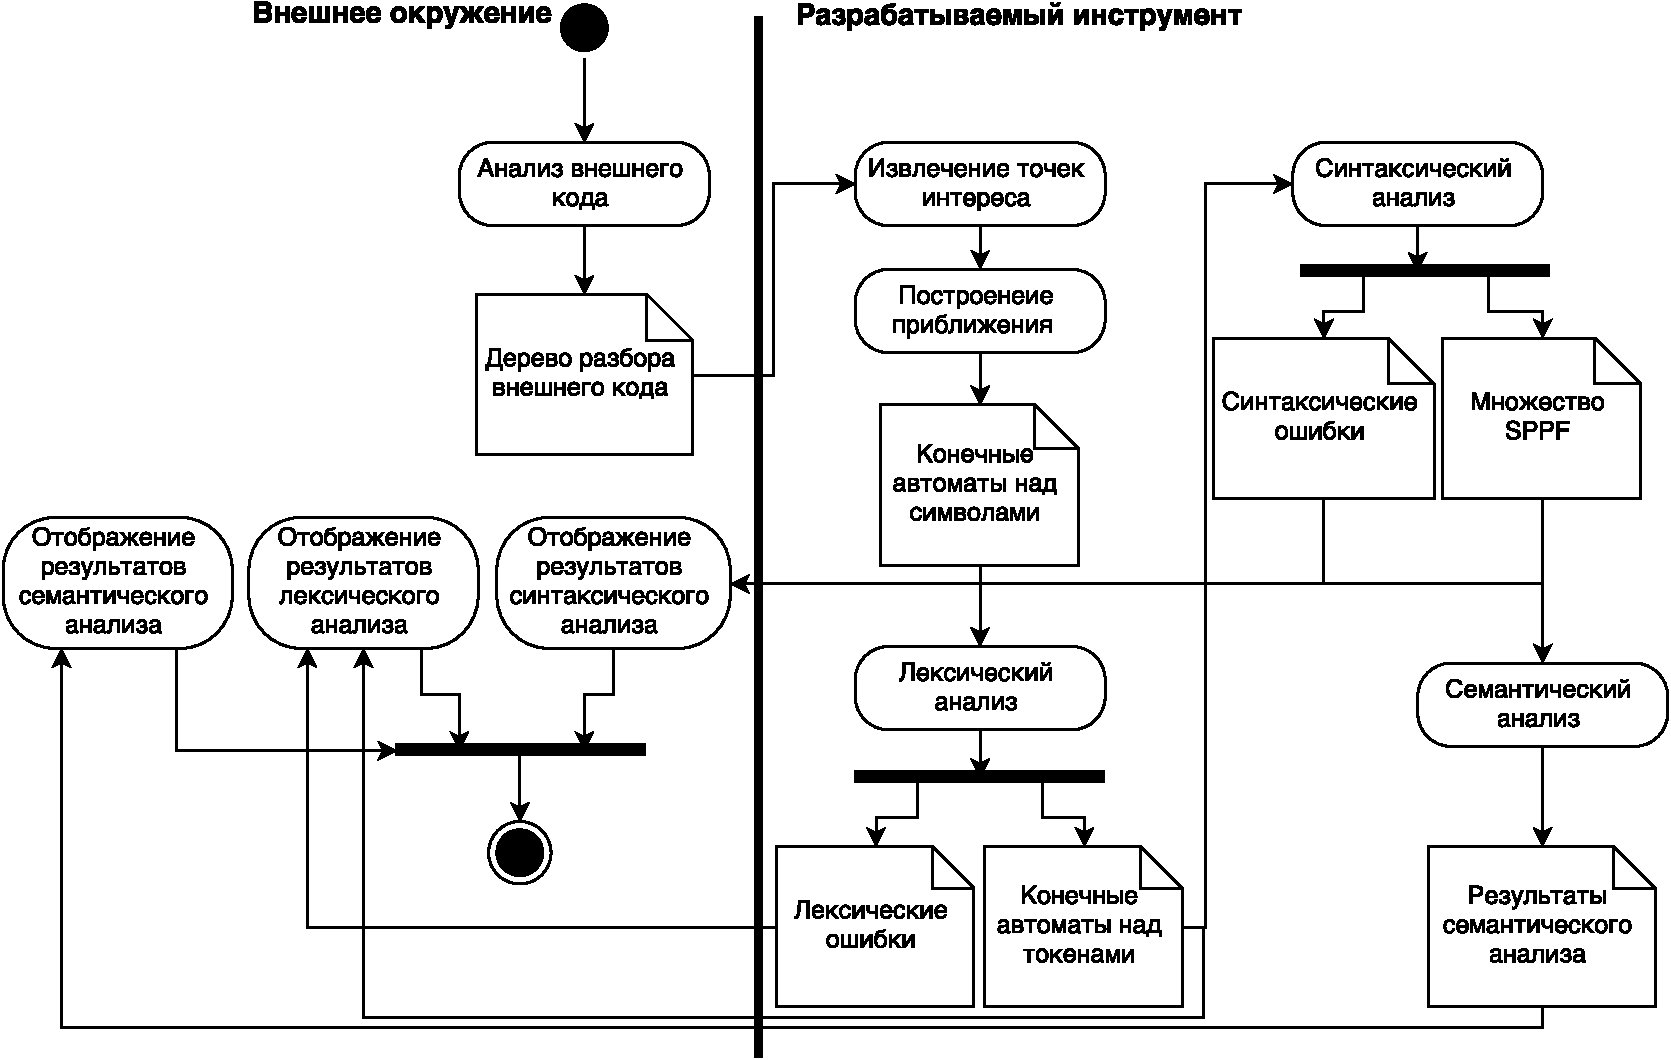
\includegraphics[width=0.9\textwidth]{pics/Activ_SEL_Processing}
\caption{Диаграмма последовательности обработки встроенных языков}
\label{fig:SeqSelProcessing} 
\end{center}
\end{figure}


Существующие инструменты для работы со встроенными языками обычно реализуют поддержку какого-то фиксированного набора языков. При этом поддержка нового языка, как правило, требует нетривиальнй доработки инструмента. Чтобы получить поддержку встроенного языка без изменений в исходном коде базового инструмента, необходимо предоставить соответствующий механизм. 

Для того чтобы упростить процесс создания конечных инструментов, создан SDK, одной из компонент которого является генератор синтаксических анализаторов на основе предложенного в данной работе алгоритма. Также в него входит генератор лексических анализаторов, библиотека построения регулярной аппроксимации, набор вспомогательных функций. Подробное описание компонент приведено далее.

Так как анализ внешнего языка является сложной самостоятельной задачей, то он не включён в разработанный SDK. На вход созданному на основе SDK инструменту должно подаваться дерево разбора внешнего языка с информацией, достаточной для решения поставленных в данной работе задач. 


\subsection{Архитектура YS.SEL.SDK}

Разработанный SDK включает компоненты, необходимые для реализации шагов, представленных на рисунке ~\ref{fig:SeqSelProcessing} и описанных ранее, за исключением анализа внешнего языка. Архитектура SDK изображена на рисунке~\ref{fig:SDKHLArch} и включает в себя генераторы анализаторов и различные библиотеки времени исполнения.

\begin{figure}[h!]
\begin{center}
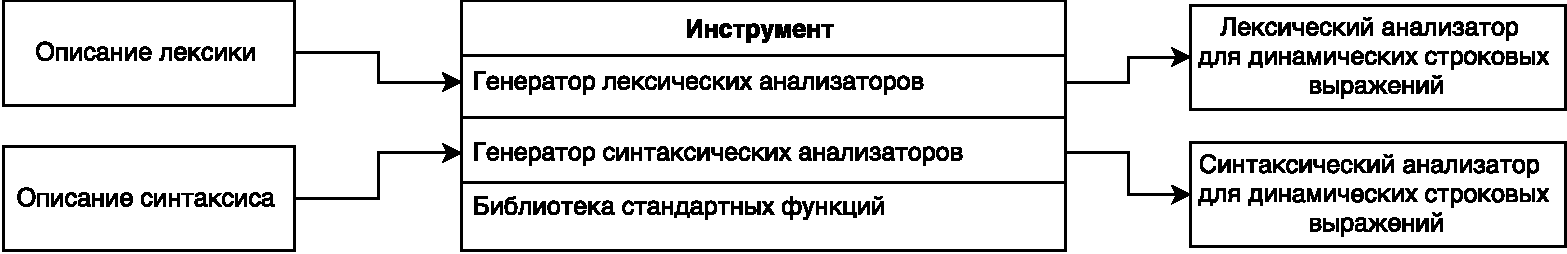
\includegraphics[width=0.9\textwidth]{pics/HighLevelArch}
\caption{Архитектура SDK целиком}
\label{fig:SDKHLArch} 
\end{center}
\end{figure}

Так как анализ внешнего языка не входит в задачи разработанного SDK, то первый шаг, выполнение которого необходимо обеспечить, --- это построение аппроксимации. В нашем случае строится регулярное приближение множества значений динамически формируемого выражения.

Построение регулярной аппроксимации основано на алгоритме, изложенном в работе~\cite{RegOverApprox}, который позволяет строить приближение сверху для множества значений выражений. То есть $L_R$, задаваемый регулярным приближением, не меньше, чем $L_1$, задаваемый программой (выполняется включение $L_R \in L_1$). Это позволяет говорить о надёжности дальнейших анализов в том смысле, что они не теряют информации о $L_1$. Например, это важно при поиске ошибок. Если в $L_R$ не обнаружено ошибок (то есть $L_R \in L_2$, где $L_2$ --- эталонный), значит и в $L_1$ ошибок нет. При этом могут быть найдены ошибки в $L_R$, которых нет в $L_1$, то есть будут ложные срабатывания. Однако наличие ложных срабатываний лучше, чем пропущенные ошибки, и их количество может быть уменьшено путём повышения точности аппроксимации. 

Для того чтобы сделать построение приближения независимым от внешнего языка, реализовано обобщённое представление графа потока управления (Control Flow Graph, CFG)~\cite{Dragon}, которое содержит всю необходимую для дальнейшей работы информацию. Таким образом, разработчику необходимо реализовать построение обобщённого представления CFG для конкретного внешнего языка. В результате компонента строит конечный автомат, являющийся приближением множества значений динамически формируемых выражений.

Архитектура компоненты, отвечающей за лексический анализ, представлена на рисунке~\ref{fig:LexArch}. Основой является  лексический анализатор, который состоит из двух частей: генератора лексических анализаторов, который по описанию лексики обрабатываемого языка, задаваемой в виде файла с расширением fsl (Lexer.fsl), строит соответствующий конечный преобразователь, и интерпретатора, который производит анализ входной структуры данных на основе построенного генератором преобразователя. Конечный преобразователь, построенный по входной спецификации, описывается с виде кода на языке F\# и сохраняется в файле (Lexer.fs). Далее данный файл может быть использован в пользовательском приложении, в рамках которого разрабатывается лексический анализатор, который устроен следующим образом. На вход принимается конечный автомат над символами, результатом работы является конечный автомат над алфавитом токенов анализируемого языка, полученный с помощью интерпретатора и преобразователя, построенного генератором. Входной конечный автомат может быть построен с помощью компоненты построения регулярной аппроксимации. Основные структуры данных --- конечный автомат и конечный преобразователь --- и функции работы с ними описаны в соответствующей библиотеке.

\begin{figure}[h!]
\begin{center}
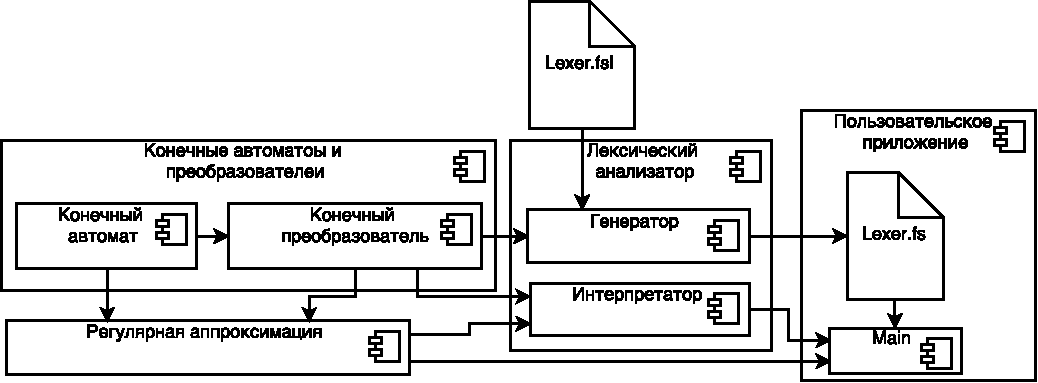
\includegraphics[width=0.95\textwidth]{pics/LexerDiagram}
\caption{Архитектура лексического анализатора}
\label{fig:LexArch} 
\end{center}
\end{figure}

Лексический анализатор реализован на основе инструмента FsLex, который является стандартным генератором лексических анализаторов для языка F\#. При реализации был переиспользован язык описания лексики и некоторые структуры данных.

Реализованный генератор лексических анализаторов обладает следующими особенностями.
\begin{itemize}
    \item Поддерживаются разрывные токены, то есть токены формируемые из нескольких строковых литералов.
    \item Сохраняется привязка лексических единиц к исходному коду: сохраняется информация о строковом литерале, из которого породился токен и координаты его внутри этой строки. Так как одна лексическая единица может формироваться из нескольких строковых литералов, то привязка сохраняется отдельно для каждой части.
    \item Поддерживается обработка входных конечных автоматов, содержащих циклы.
    \item Так как значение токена может формироваться с помощью цикла и, как следствие, быть бесконечным, то каждый токен содержит конечный автомат, порождающий все возможные значения для данного токена, а не единственное значение, как это реализовано в классическом лексическом анализе.
\end{itemize}

\textbf{Генератор синтаксических анализаторов}, названный ARNGLR, реализован на основе алгоритма, описанного в разделе~\ref{AlgoDescr}. Его архитектура представлена на рисунке~\ref{fig:ParsArch}.  

\begin{figure}[h!]
\begin{center}
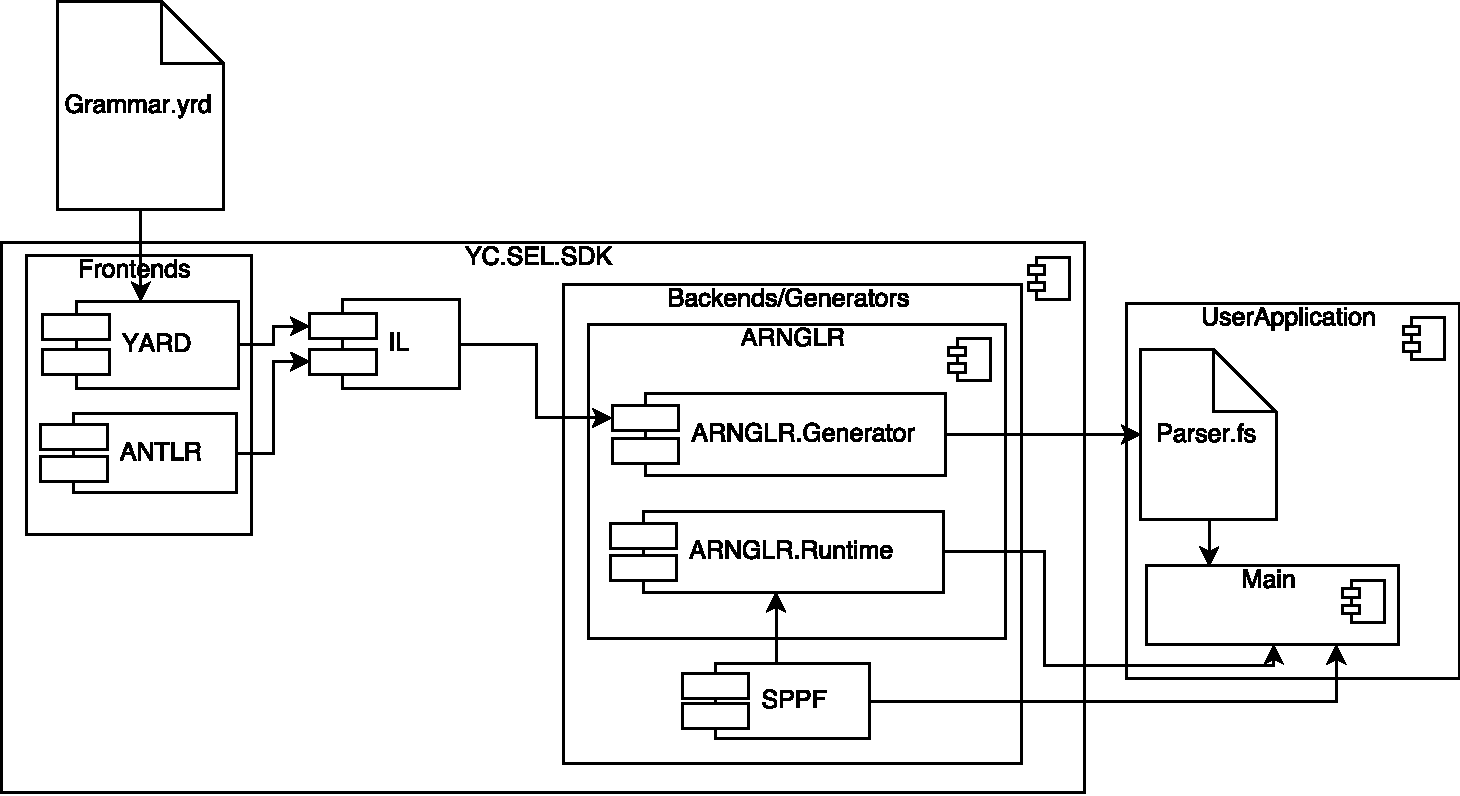
\includegraphics[width=0.95\textwidth]{pics/ARNGLRArch}
\caption{Архитектура синтаксического анализатора}
\label{fig:ParsArch} 
\end{center}
\end{figure}

Генератор реализован как один из модулей YC и может принимать на вход внутреннее представление грамматики (IL), которое может быть получено с помощью различных фронтендов (Frontends), однако в рамках YC.SEL.SDK 
основным фронтендом является YARD, так как он предоставляет наиболее развитые средства для описания грамматик. По грамматике обрабатываемого языка строятся управляющие таблицы анализатора, которые сохраняются в файле Parser.fs. 
Построенные таблицы должны быть включены в разрабатываемое приложение UserApplication. Интерпретатор, предназначенный для синтаксического разбора конечного автомата, полученный после лексического анализа, реализован 
в виде отдельной библиотеки ARNGLR.Runtime, которая также должна быть подключена к разрабатываемому приложению. В результате работы интерпретатора будет получен SPPF, который может быть использован для дальнейшей 
обработки (например, подсчёта метрик). Для упрощения работы с SPPF реализован ряд вспомогательных функций.

\subsection{Архитектура YC.SEL.SDK.ReSharper}

ReSharper --- это расширение к Microsoft Visual Studio IDE, предоставляющее широкий спектр  дополнительной функциональности по анализу и рефакторингу кода. ReSharper поддерживает несколько языков, например C\#, Visual Basic .NET, JavaScript, и этот список может быть расширен благодаря наличию свободно распространяемого ReSharper SDK, описание которого было представлено ранее в разделе~\ref{ReSharperSDKDescr}. ReSharper.SDK позволяет получить деревья разбора для поддерживаемых языков, предоставляет набор готовых анализов и упрощает взаимодействие с Microsoft Visual Studio IDE и её компонентами. Более того, предоставляется возможность разработки собственных расширений для ReSharper на основе ReSharper.SDK.

Microsoft Visual Studio является достаточно распространённой средой разработки, но не поддерживает встроенные языки, поэтому было решено разработать ряд расширений к ReSharper с использованием разработанного инструментария, которые будут устранять данный недостаток. Стоит отметить, что не ставилось задачи поддержать все встроенные языки, так как встроенным может быть любой язык программирования. Также не было необходимости поддержать все внешние языки программирования. Необходимо на базе разработанного YC.SEL.SDK создать инфраструктуру, позволяющую реализовывать поддержку новых встроенных языков в Microsoft Visual Studio через расширения к ReSharper и реализовать несколько расширений, демонстрирующих возможности созданной инфраструктуры. 

Так как необходимо поддерживать различные языки, то необходимо обеспечить расширяемость по новыми языками. Классический подход к решению такой задачи для интегрированных сред разработки заключается в том, что поддержка нового языка реализуется в виде независимой компоненты. Если пользователь хочет получить поддержку какого-либо языка в своей среде разработки, то он должен установить соответствующий пакет. При этом поддержка различных языков осуществляется независимо, однако часто выделяется общая функциональность, которая может быть оформлена в виде отдельного пакета.

Для предоставления описанных выше возможностей была реализована надстройка над YC.SEL.SDK, упрощающая создание расширений для ReSharper, названная  YC.SEL.SDK.ReSharper. В неё включены компоненты, реализующие функции, которые упрощающают взаимодействие YC.SEL.SDK и ReSharper.SDK. Назначени основных из них описаны ниже.

\begin{itemize}
  \item Общая точка расширения, необходимая для подключения функциональности для различных встроенных языков, которая может быть реализована в различных расширениях, к ReSharper через общий интерфейс. Также общая точка расширения позволяет использовать общую функциональность, необходимую для работы со встроенными языками.
  \item Отображение в IDE информации, полученной в ходе анализа. Например, подсветка синтаксиса и ошибок. Вывод диагностических сообщений с информацией об ошибках.
  \item Преобразование данных, из формата, используемого в ReSharper.SDK, в формат для YC.SEL.SDK. Например, преобразование графа потока управления внешнего языка, построенного ReSharper.SDK, в формат, пригодный для построения регулярной аппроксимации средствами YC.SEL.SDK.
  \item Управление работой анализаторов, необходимое, с одной стороны, для обеспечения своевременной реакции на изменения в коде, совершённые пользователем, а с другой, для прекращения вычислений, результаты которых уже не актуальны. Управление построено на основе общего для ReSharper механизма, обеспечивающего асинхронную работу анализов. При этом вычисления могут быть прерваны, если, например, пользователь внёс в код изменения, делающие анализ или его результаты некорректными. 
\end{itemize}

Как уже говорилось, встроенными могут быть различные языки и учесть заранее все их особенности не представляется возможным. Кроме того, даже при использовании одного встроенного языка могут использоваться различные способы выполнения сформированного запроса. Таким образом, необходимо предоставлять возможность настройки расширений конечным пользователем. Для этого в рамках YC.SEL.SDK.ReSharper была реализована возможность управления следующими основными параметрами расширений. 

\begin{itemize}
    \item Подсветка синтаксиса для каждого языка. Предоставлена возможность указать цвет для каждого типа токена.
    \item Указание парных элементов. Для каждого языка можно указать, какие лексические единицы считать парными: для каждой пары указывается ``левый'' (открывающая скобка) и ``правый'' (закрывающая скобка) элементы. При расположении курсора в тексте рядом с одним из элементов пары будут подсвечены соответствующие элементы. Пример подсветки парных элементов приведён на рисунке~\ref{fig:braces}.
    \item Точки интереса или хотспоты (hotspot) --- это места, в которых должно быть сформировано финальное выражение. Необходимо знать, какой хотспот какому языку соответствует. При этом нужно учитывать, что одному языку может соответствовать несколько хотспотов. Например, динамически сформированный SQL-запрос в программе на языке программирования C\# может быть выполнен с помощью метода \verb|ExecuteQuery| класса \verb|DataContext|~\cite{ExecuteQuery}
     или же текст запроса может быть передан как аргумент конструктора класса \verb|SqlCommand|~\cite{SqlCommand} с последующим выполнением с помощью метода \verb|ExecuteReader|.

\end{itemize}

Настройка указанных выше параметров хранится в соответствующих конфигурационных файлах в формате XML, которые на данный момент редактируются вручную. Настройка подсветки синтаксиса и парных элементов совмещена в одном файле и для каждого языка создаётся отдельный такой файл. Конфигурационный файл с точками интереса является общим для всех языков и, соответственно, для всех установленных расширений для поддержки встроенных языков.

В листинге~\ref{lst:codeHighlighting} приведён пример конфигурации подсветки синтаксиса и парных скобок для языка Calc. Для указания цвета используются имена, принятые в ReSharper (например, \verb|"CONSTANT_IDENTIFIER_ATTRIBUTE"|), что должно сделать настройку цветов более единообразной. В xml-тэге \verb|Matched| содержится описание парных элементов. Каждая пара описывается в xml-тэге \verb|Pair| и для одного языка может быть указано более одной такой пары.

\fvset{frame=lines,framesep=5pt}
\begin{listing}[H]
    \begin{pyglist}[language=xml,numbers=left,numbersep=5pt]
<?xml version="1.0" encoding="utf-8"?>
<SyntaxDefinition name="CalcHighlighting">
    <Colors>
        <Tokens color="CONSTANT_IDENTIFIER_ATTRIBUTE">
            <Token> DIV </Token>
            <Token> LBRACE </Token>
            <Token> MINUS </Token>
            <Token> MULT </Token>
            <Token> NUMBER </Token>
            <Token> PLUS </Token>
            <Token> POW </Token>
            <Token> RBRACE </Token>
        </Tokens>
    </Colors>
<!-- Dynamic highlighting: -->
    <Matched>
        <Pair>
            <Left> LBRACE </Left>
            <Right> RBRACE </Right>
        </Pair>
<!-- You can specify more then one pair:        
        <Pair>
            <Left> LEFT_SQUARE_BRACKET </Left>
            <Right> RIGHT_SQUARE_BRACKET </Right>
        </Pair>
        <Pair>
            <Left> LEFT_FIGURE_BRACKET </Left>
            <Right> LEFT_FIGURE_BRACKET </Right>
        </Pair>
-->        
    </Matched>
</SyntaxDefinition>
    \end{pyglist}
\caption{Пример конфигурационного файла для настройки подсветки синтаксиса}
\label{lst:codeHighlighting}
\end{listing}

Листинг~\ref{lst:hotspots} содержит пример описания точек интереса. Для каждой точки интереса должна быть указана следующая информация.
\begin{itemize}
    \item Какому встроенному языку соответствует точка. Информация хранится в Xml-тэге \verb|Language|.
    \item Полное имя метода, являющегося точкой интереса. Информация хранится в Xml-тэге \verb|Method|.
    \item Порядковый номер аргумента данного метода, являющегося выражением на встроенном языке. Нумерация начинается с нуля. Информация хранится в Xml-тэге \verb|ArgumentPosition|. 
    \item Возвращаемый тип метода.  Информация хранится в Xml-тэге \verb|ReturnType|. 
\end{itemize}

\fvset{frame=lines,framesep=5pt}
\begin{listing}[H]
    \begin{pyglist}[language=xml,numbers=left,numbersep=5pt]
<?xml version="1.0" encoding="utf-8"?>
<!-- comment about body -->
<Body>
    <!-- comment about hotspot -->
  <Hotspot>
      <!-- comment about tsql -->
      <Language> TSQL </Language>
      <!-- comment about fullName -->
      <Method>Program.ExecuteImmediate</Method>
      <!-- zero-based -->
      <ArgumentPosition> 0 </ArgumentPosition>
      <!-- comment about return type -->
      <ReturnType> void </ReturnType>
  </Hotspot>
  <Hotspot>
      <Language> Calc </Language>
      <Method>Program.Eval</Method>
      <ArgumentPosition> 0 </ArgumentPosition>
      <ReturnType> int </ReturnType>
  </Hotspot>
</Body>
    \end{pyglist}
\caption{Пример конфигурационного файла для настройки точек интереса}
\label{lst:hotspots}
\end{listing}


\section{Области и способы применения YC.SEL.SDK}

Разработанный SDK предназначен для создания инструментов статического анализа динамически формируемых строковых выражений. Решения, созданные с его помощью, могут применяться для работы с проектами, активно использующими динамически формируемые строковые выражения. Необходимость работать с такими проектами может возникнуть, например, в следующих областях.

\begin{itemize}
    \item Реинжиниринг программного обеспечения.
    \item Поддержка встроенных языков в средах разработки.
    \item Оценка качества и сложности кода.
\end{itemize}

Общим для всех этих областей является то, что для решения многих задач необходимо структурное представление динамически формируемого кода. При этом анализируемые языки могут быть различными и процесс их анализа часто тесно связан с анализом внешнего языка.

Отметим, что встроенные языки используются всё менее активно в молодых проектах и системах. На смену им приходят более надёжные способы композиции языков и метапрограммирования. Например LINQ или ORM-технологии. Однако это не всегда так. Использование строковых выражений для взаимодействия с базами данных и генерации WEB-страниц в приложениях на PHP всё ещё широко распространено~\cite{DSQLInActiveUse}. Это необходимо учитывать при поддержке встроенных языков в средах разработки. Для каких-то языков на первый план выходят возможности по изучению и модификации уже созданного кода, а для каких-то --- возможность быстро и удобно создавать новый код. Во втором случае могут возникнуть дополнительные требования к скорости работы инструмента, так как подразумевается выполнение некоторых операций ``на лету'', что может послужить ограничением на использование SDK, так как многие механизмы, реализованные в нём, не предусматривают возможности уменьшения точности в пользу увеличения быстродействия. Оценка качества и сложности  кода часто может выполняться в рамках комплекса задач по реинжинирингу системы, однако может быть и самостоятельной задачей, например, при оценке сложности работ по поддержке и сопровождению информационной системы.

Детали применения SDK могут варьироваться в зависимости от решаемых задач и контекста использования. Например, механизм построения регулярной аппроксимации может быть реализован независимо в рамках внешнего инструмента. Однако основной сценарий использования аналогичен использованию инструментариев для разработки компиляторов. Последовательность шагов, представленная ниже, может быть изменена в зависимости от особенностей задачи.

\textbf{Шаг 1.} Создание грамматики обрабатываемого языка. Грамматика может быть создана на основе документации соответствующего языка или переиспользована готовая, что оправданно, например, при создании анализатора для динамического SQL, когда внешний и встроенный языки совпадают.

\textbf{Шаг 2.} Генерация синтаксического анализатора по созданной грамматике. Для этого используется генератор синтаксических анализаторов, присутствующий в SDK. Результатом работы генератора является файл с исходным кодом на языке программирования F\#, который должен быть включён в разрабатываемый код. Файл содержит описание типов для лексических единиц, управляющие таблицы анализатора и функцию, которая по конечному автомату над алфавитом токенов анализируемого языка построит SPPF, содержащий деревья вывода всех корректных цепочек.

\textbf{Шаг 3.} Создание лексической спецификации обрабатываемого языка. Спецификация может быть извлечена из документации или заимствована из других проектов. При обработке динамически формируемого SQL возможно переиспользовать спецификацию, созданную для основного языка, которым также является SQL. При этом необходимо обратить внимание на то, что типы лексических единиц определяются на основе созданного на предыдущих шагах синтаксического анализатора.

\textbf{Шаг 4.} Генерация лексера по созданной спецификации. Для этого применяется генератор лексических анализаторов, входящий в состав SDK. В результате его применения получается файл с исходным кодом на языке F\#, который должен быть подключён к разрабатываемому решению. 

\textbf{Шаг 5.} Реализация механизма построения регулярной аппроксимации, результатом которого является функция, строящая конечный автомат над алфавитом символов. Данный механизм может быть реализован либо на основе предоставляемого в рамках SDK, либо независимо. В первом случае от разработчика требуется построить обобщённый CFG для внешнего языка. Во втором случае необходимо только гарантировать правильность возвращаемого конечного автомата. Второй подход может быть использован, например, при наличии реализованного механизма протягивания констант для внешнего языка. Это позволит создать возможно менее точное, но, скорее всего, более быстрое построение аппроксимации. Такой подход применим при автоматизированном реинжиниринге, когда ручная доработка кода является обязательным шагом и абсолютная точность автоматической обработки не требуется. Ещё одна возможная область применения второго подхода --- это поддержка встроенных языков в средах разработки. Здесь также часто не требуется высокая точность для подсказок пользователю, однако производительность крайне важна. Поэтому иногда приходится жертвовать точностью анализа для достижения нужной скорости работы.

\textbf{Шаг 6.} Реализация работы с SPPF. Синтаксический анализатор возвращает SPPF --- конечное представление леса разбора всех корректных цепочек из аппроксимации. Дальнейшая работа с ним может строиться по двум основным сценариям.

Превый сценарий --- непосредственная обработка SPPF. В этом случае все вычисления происходят над SPPF без извлечения отдельных деревьев. Это позволит ускорить обработку результатов разбора, так как количество деревьев может быть бесконечным, а SPPF является конечной структурой данных. Однако существует несколько проблем, связанных с таким подходом. Во-первых, требуется создание новых процедур обработки, так как классические, как правило, ориентированы на работу с деревьями. Во-вторых, могут возникнуть трудности при выполнении некоторых анализов, вызванные тем, что в SPPF хранятся ``бесконечные'' деревья. Например, необходимо вычислить максимальную глубину вложенности конструкции \verb|if|, являющуюся одной из стандартных метрик сложности кода. SPPF может содержать 
циклы и может оказаться так, что конструкция \verb|if| встречается в цикле таким образом, что потенциальная глубина вложенности может быть бесконечной. Такая ситуация не является стандартной при 
обработке деревьев разбора и её надо отслеживать отдельно.

Второй сценарий --- извлечение отдельных деревьев из SPPF и их обработка. Данный подход может оказаться удобным, если уже существуют процедуры обработки синтаксических деревьев для языка, который оказался встроенным. Это помогает избежать затрат на создание новой функциональности. Такое может произойти при работе с динамическим SQL. В этом случае для работы с деревом разбора внешнего языка и деревьями, извлечёнными из SPPF, можно использовать одни и те же процедуры, так как языки идентичны.

Недостатком второго подхода является то, что конечность числа деревьев не гарантирована. Это значит, что не удастся обработать все деревья. Стоит отметить, что даже в случае конечности числа деревьев, перебор и обработка всех деревьев разбора может потребовать значительных ресурсов.


\textbf{Шаг 7.} Реализация механизмов сбора, обработки и отображения информации, такой как сообщения об ошибках или любой другой, полученной в процессе анализа. Необходимо для предоставления пользователю информации, ожидаемой в рамках решаемой задачи.

На рисунке~\ref{fig:activMethod} изображён один из возможных сценариев использования SDK. Особенностью является цикличность процесса, характерная, например для реинжиниринга программного обеспечения.

\begin{figure}[h!]
\begin{center}
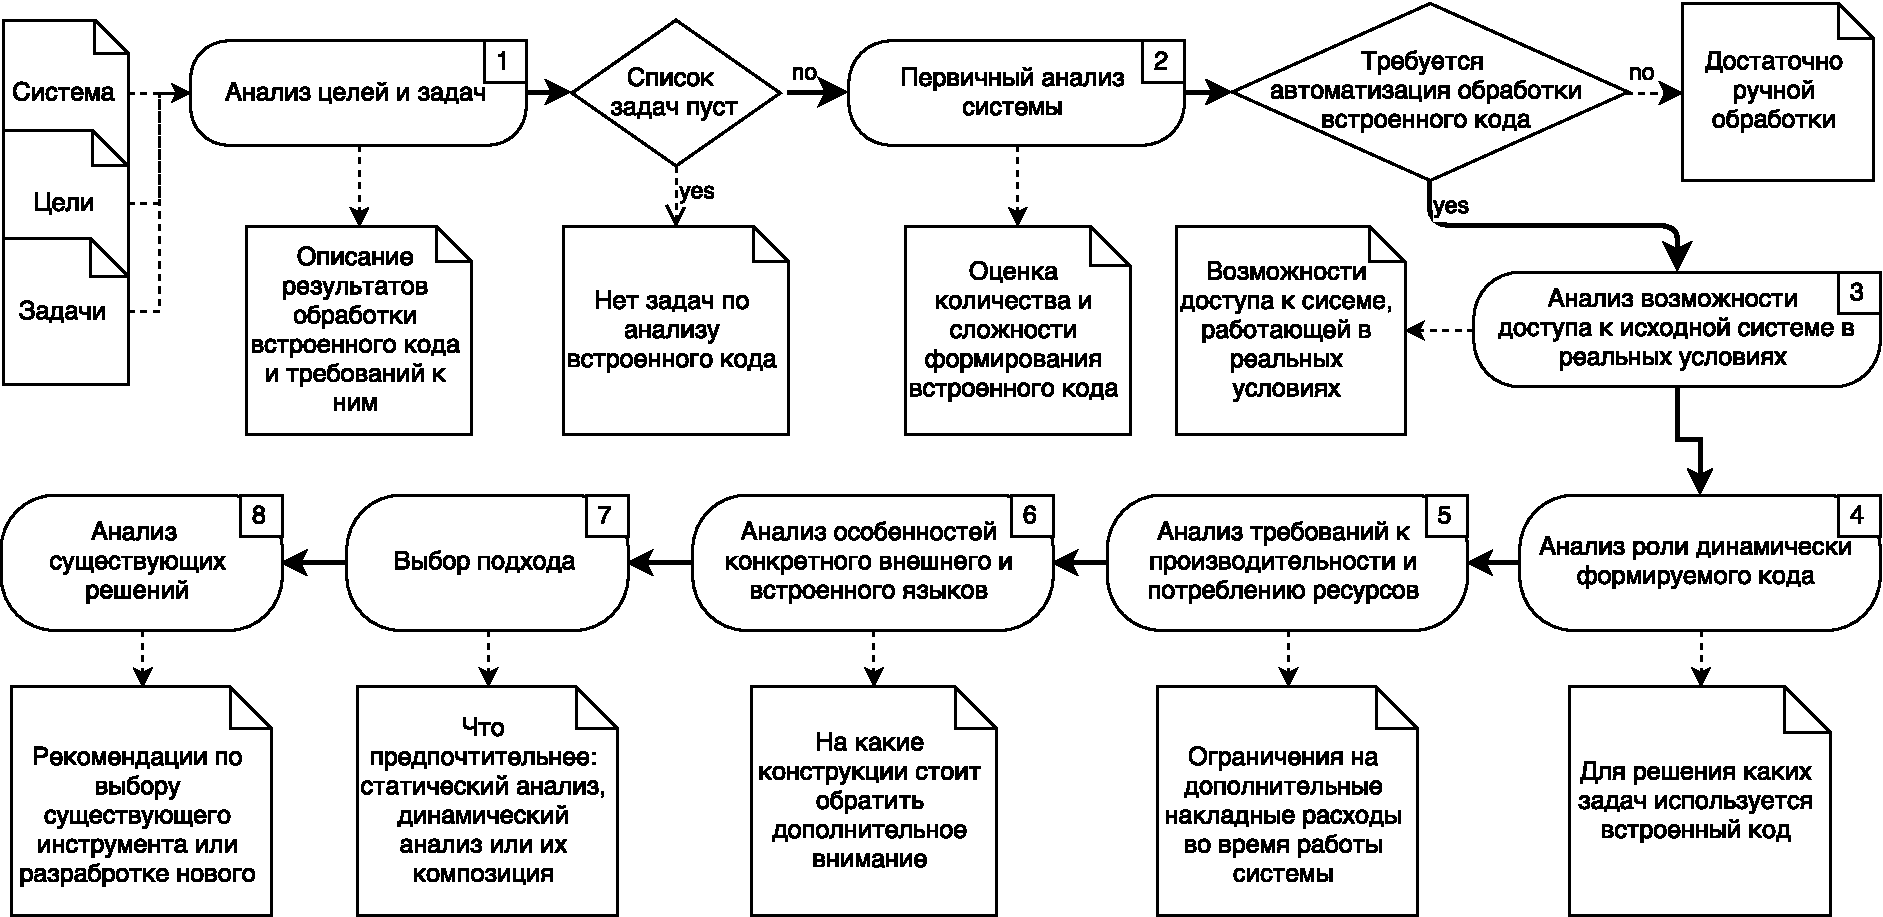
\includegraphics[width=0.9\textwidth]{pics/ActivMethodology}
\caption{Один из возможных вариантов использования SDK в проектах по реинжинирингу}
\label{fig:activMethod} 
\end{center}
\end{figure}

Встраивание анализа строковых выражений в последовательность обработки кода всей системы зависит от решаемых задач. Первыми шагами идут действия, необходимые для того, чтобы получить входные данные для анализа. Для этого необходимо провести лексический и синтаксический анализ внешнего языка, построить граф потока управления. После этого возможно построение аппроксимации и дальнейший анализ встроенных языков. Параллельно с этим может проводиться дальнейшая обработка внешнего языка. Степень параллельности зависит от независимости решаемых задач. Например, некоторые метрики сложности для основного кода и для динамически формируемого можно считать независимо и выводить отдельно. С другой стороны, может возникнуть необходимость вычислить некую комплексную метрику, учитывающую параметры и внешнего и динамически формируемого кода, что приведёт к необходимости синхронизации.

\section{Особенности реализации}

Разработка инструментального пакета с описанной выше архитектурой и плагинов для ReSharper велась в рамках исследовательского проекта YaccConstructor (YC), описанного в разделе~\ref{YCDescr}. 
Разработка велась на платформе .NET и основной язык реализации --- F\#~\cite{FSharp}. Весь исходный код опубликован на GitHub~\cite{YCUrl}. 
Большинство компонент опубликовано под ``открытой'' лицензией Apache License Version~2.0~\cite{ApacheV2}. 

За основу алгоритма синтаксического анализа динамически формируемых выражений был взят реализованный в YC алгоритм синтаксического анализа RNGLR. Генератор управляющих таблиц был использован практически без 
модификаций, а интерпретатор был реализован отдельный. Кроме этого, общими являются некоторые структуры данных и вспомогательные функции, такие как представление леса разбора и его печать в формате 
DOT~\footnote{DOT --- текстовый язык описания графов~\cite{DOT}.}, представление GSS. 

Лексичекий анализ реализован на основе инструмента FsLex, который потребовал значительных доработок для того, чтобы обеспечить обработку конечного автомата, а не линейного входа. Все остальные компоненты, 
необходимые для статического анализа динамически формируемых выражений, такие как построение аппроксимации, вспомогательные функции для упрощения построения целевых инструментов были реализованы ``с нуля'' 
в рамках проекта YC.

Бинарные пакеты, содержащие основную функциональность, опубликованы в сети интернет на NuGet~\footnote{NuGet --- менеджер пакетов для платформы .NET и одноимённый ресурс для их публикации. Позволяет публиковать 
и устанавливать пакеты, автоматически отслеживать зависимости между ними~\cite{NuGet}.}.


\clearpage
\section{Эксперименты}

Был проведён ряд экспериментов, которые позволили оценить некоторые параметры инструмента.

Во всех приведённых ниже тестах грамматики описываются на языке YARD. Так же предположим, что у нас есть сторонний лексический анализатор со следующим набором лексем:
\begin{itemize}
  \item PLUS = '+'
  \item MINUS = '-'
  \item DIV = '/'
  \item MULT = '*'
  \item LEFT = '('
  \item RIGHT = ')'
  \item NUMBER = (0..9)+
  \item SEMICOLON = ';'
\end{itemize}

По этому будем предполагать, что на вход инструменту поступает поток лексем.


\subsection{Работа с однозначными грамматиками} 

Необходимо показать, что по однозначной грамматике строится инструмент имеющий линейную временную сложность. Для этого необходимо оценить количество действий LR-автомата, совершаемых при распознавании цепочки. Оно должно линейно зависеть от длинны входа.

В нашем случае операции LR-автомата -- это вызовы функций $parse$ и $climb$. То есть нам надо оценить зависимость количества вызовов этих функций от длинны входной цепочки.


Возьмём грамматику:

\begin{verbatim}
f : <n:string>=NUMBER {float n}
  | l=LEFT <expr:float>=e r=RIGHT {expr};  
  
t : <l:float>=t op=(MULT {( * )} | DIV {( / )} ) <r:float>=f {op l r}
  | res=f {res};
  
e : res=t {res}
  | <l:float>=e op=(PLUS {( + )} | MINUS {( - )} ) <r:float>=t {op l r}; 
  
+s: res=e {res};
\end{verbatim}

Возьмём n = "`2*3"' и проведём тесты для строк n'+'kn, kn = $concat \ '\!+' [\underbrace {n,n, ... , n}_\text{k раз}] | k = 0..99 $. В результате получим график~\ref{fig:assimpt}, где по оси Ox откладывается k, а по Oy -- количество вызовов. Видно, что зависимость количества действий LR-автомата линейно зависит от длины входной цепочки.

\begin{center}
  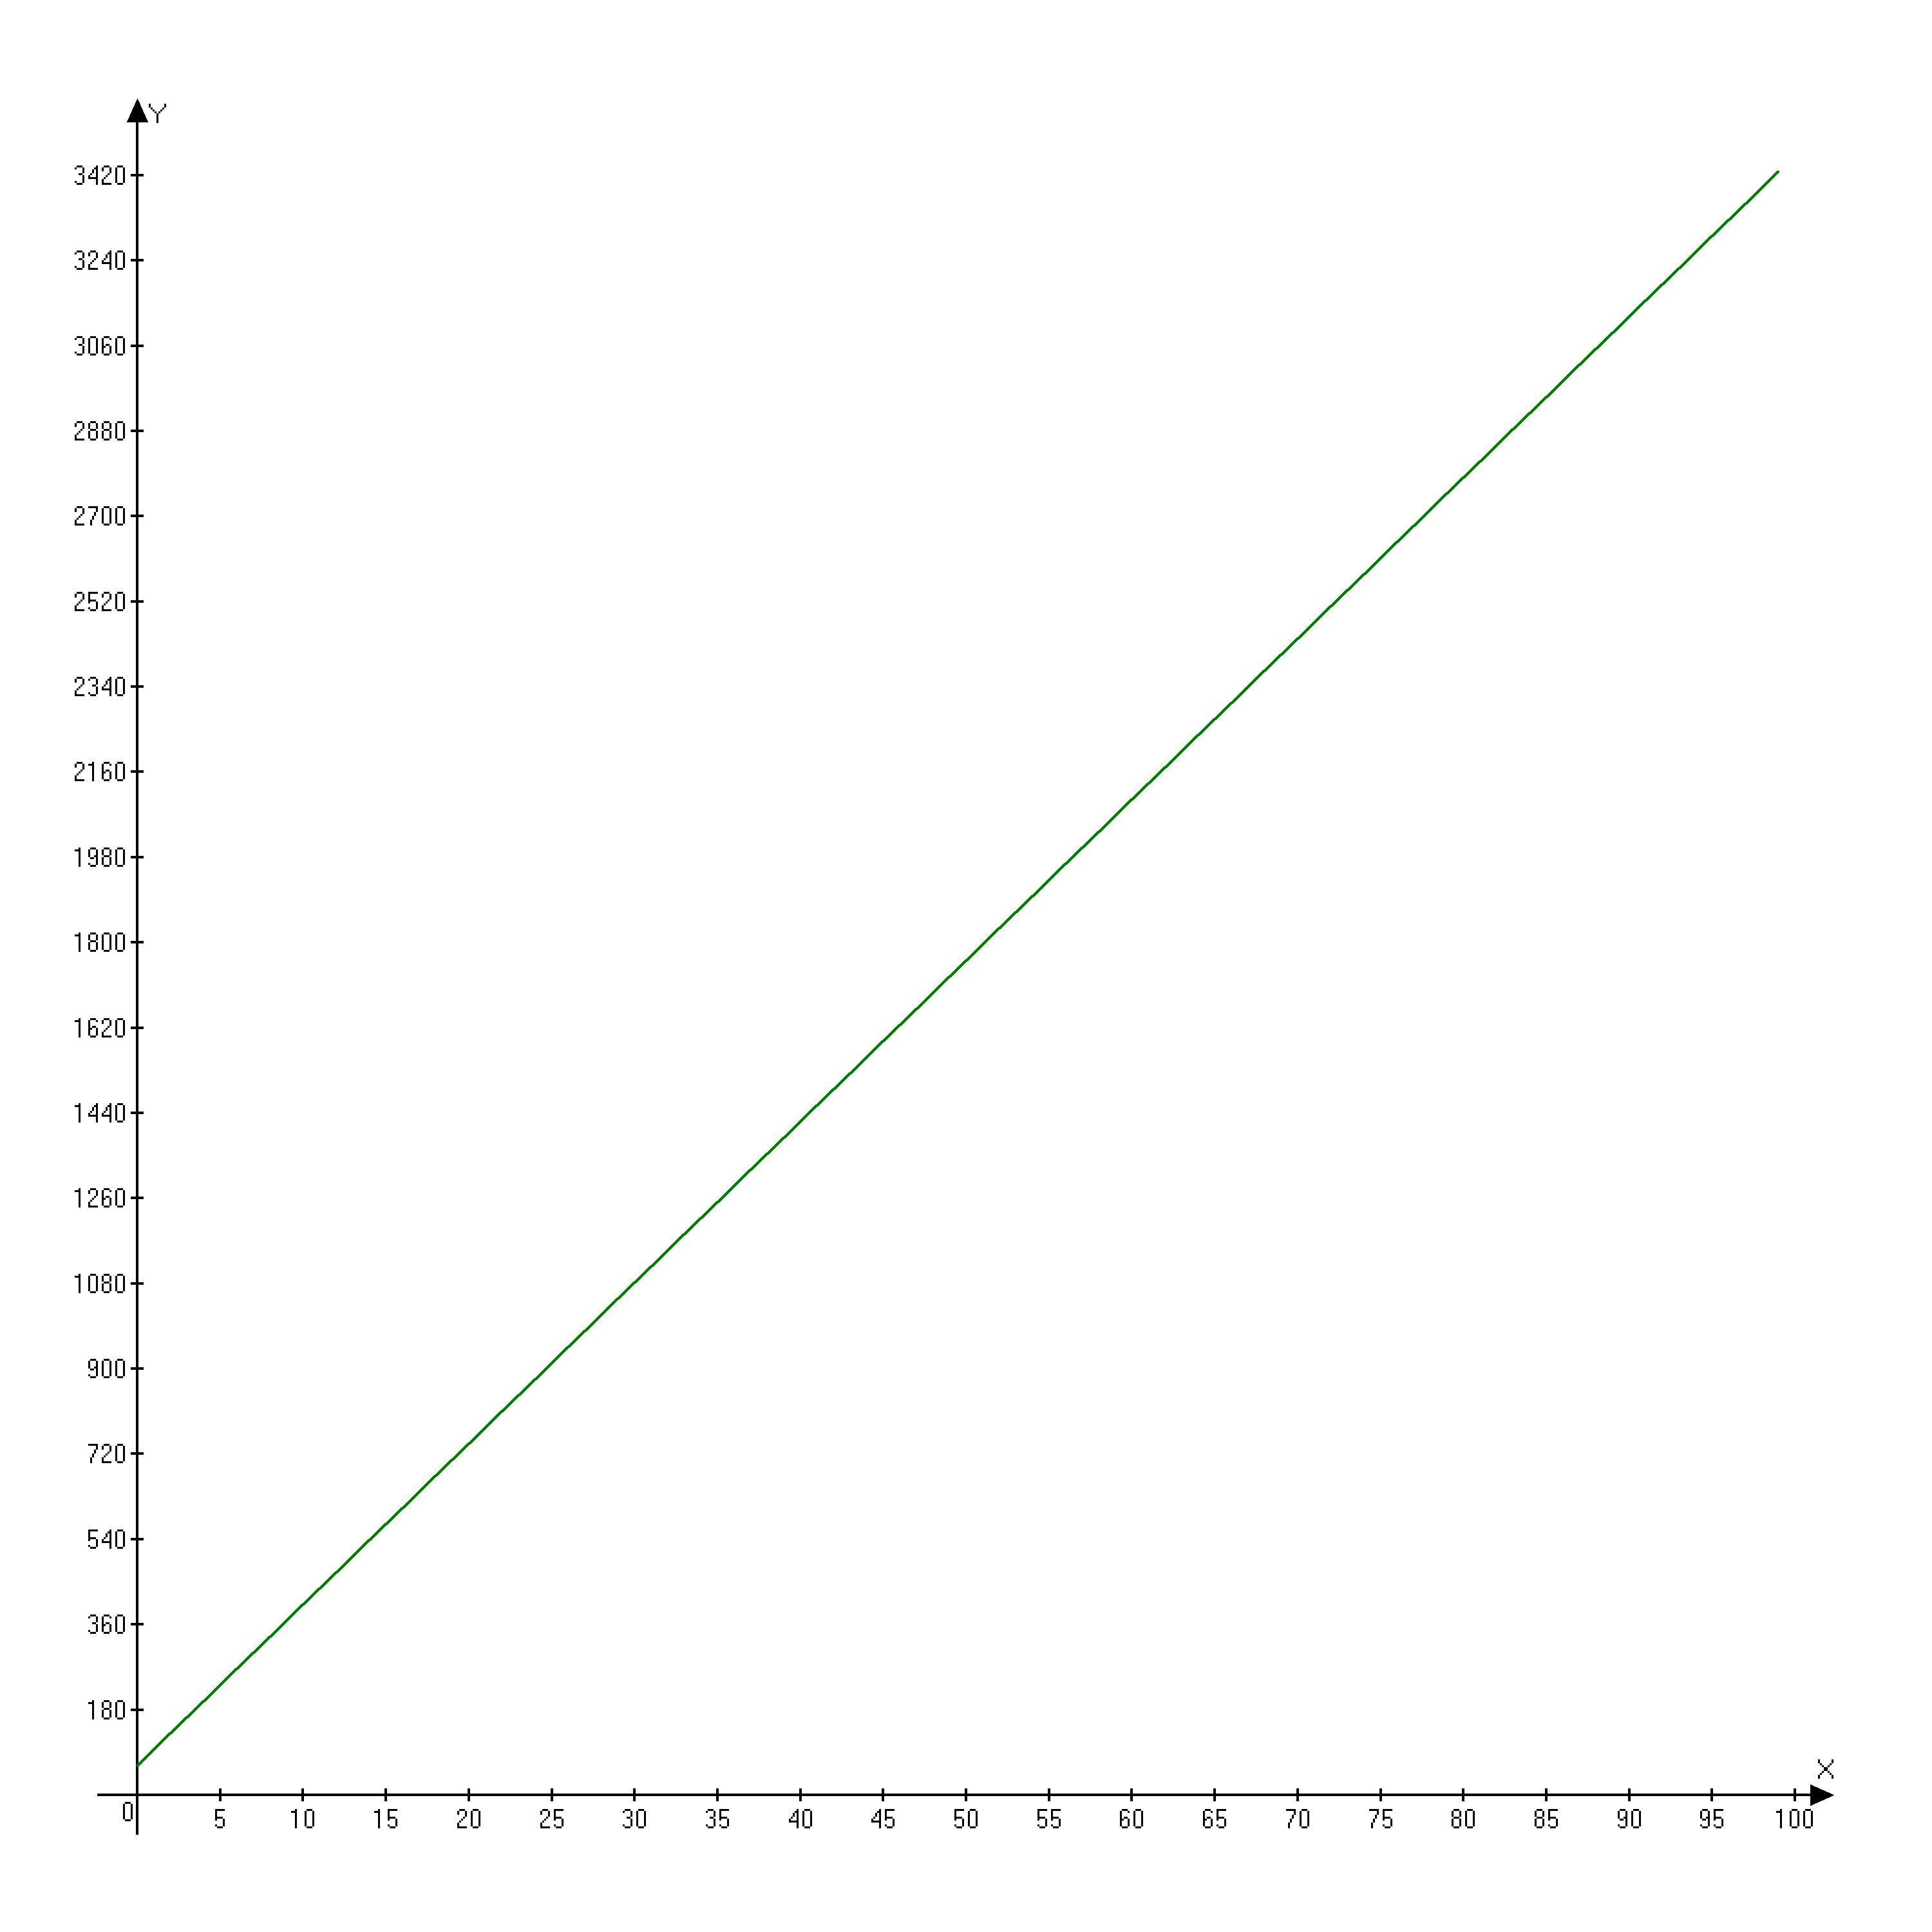
\includegraphics[height = 15cm]{Pictures/CallCount_18.jpg} 
	\captionof{figure}{Зависимость количества действий LR-автомата от длинны входной цепочки.}
	\label{fig:assimpt}
\end{center}


\subsection{ Возможность работы с неоднозначными грамматиками} 

Для этого необходимо проверить, что при неоднозначной грамматике инструмент возвращает все возможные варианты вывода входной строки. В качестве примера была взята следующая грамматика:

\begin{verbatim}
+s : e;
e : e (PLUS | MINUS | MULT | DIV  ) e 
  | LEFT e RIGHT 
  | NUMBER ;
\end{verbatim}

Эта грамматика описывает арифметические выражения без приоритетов. Очевидно, что данная грамматика содержит неоднозначности. 

Рассмотрим несколько примеров входных цепочек:
\begin{itemize}

  \item Пусть тестовая строка: "`1+2"'. Соответсвенно, список лексем: \verb|[NUMBER; PLUS; NUMBER]|. Существует единственное дерево вывода для данной цепочки:

    \begin{centering}

      \begin{dot2tex}[dot]
       digraph g
       {
          S [label = "S"]
          e1 [label = "e"]
          e2 [label = "e"]
          plus [label = "PLUS"]
          e3 [label = "e"]
          num1 [label = "NUMBER"]
          num2 [label = "NUMBER"]
          S -> e1
          e1 -> e2
          e1 -> plus
          e1 -> e3
          e2 -> num1
          e3 -> num2
       }
      \end{dot2tex}

    \end{centering}

Инструмент так же возвращает единственное дерево:
\begin{verbatim}
<NODE name="S">
        <NODE name="e">
            <NODE name="e">
                <LEAF name="NUMBER"/>
            </NODE>
            <LEAF name="PLUS"/>
            <NODE name="e">
                <LEAF name="NUMBER"/>
            </NODE>
        </NODE>
</NODE>
\end{verbatim}

\item Строка: "`1+2+3"'. Список лексем: \verb|[NUMBER; PLUS; NUMBER; PLUS; NUMBER]|. Для данной цепочки существует два дерева вывода и инструмент возвращает оба:
\begin{verbatim}
<NODE name="s">
    <NODE name="e">
        <NODE name="e">
            <NODE name="e">
                <LEAF name="NUMBER"/>
            </NODE>
            <LEAF name="PLUS"/>
            <NODE name="e">
                <LEAF name="NUMBER"/>
            </NODE>
        </NODE>
        <LEAF name="PLUS"/>
        <NODE name="e">
            <LEAF name="NUMBER"/>
        </NODE>
    </NODE>
</NODE>

<NODE name="s">
    <NODE name="e">
        <NODE name="e">
            <LEAF name="NUMBER"/>
        </NODE>
        <LEAF name="PLUS"/>
        <NODE name="e">
            <NODE name="e">
                <LEAF name="NUMBER"/>
            </NODE>
            <LEAF name="PLUS"/>
            <NODE name="e">
                <LEAF name="NUMBER"/>
            </NODE>
        </NODE>
    </NODE>
</NODE>
\end{verbatim}
	
\end{itemize}
	
Таким образом, инструмент строит все возможные варианты вывода в случае, если грамматика неоднозначна.

\subsection{Возможность работы с EBNF-грамматиками} 

Основные конструкции регулярных выражений, для которых необходимо провести проверку: последовательность, альтернатива, замыкание. Важно обратить внимание на соответствие получаемого дерева вывода ожидаемому результату. Для этого нужно проверить соответствие дерева вывода входной грамматике. В нём не должно быть новых терминалов и нетерминалов.

Для примера возьмём следующую грамматику:
\begin{verbatim}
f : NUMBER 
  | LEFT e RIGHT ;  
  
t : t (MULT | DIV ) f 
  | f ;
  
e : t 
  | e (PLUS | MINUS )t; 
  
+s: e (SEMICOLON e )* ;

\end{verbatim}

Данная грамматика описывает список арифметических выражений, разделённых точкой с запятой. Видно, что в ней используются все заявленные конструкции регулярных выражений (последовательность, альтернатива, замыкание).

Пусть на вход подаётся строка: "`2*3; 3*4; 5*5"'. Инструмент построит следующее дерево вывода:
\begin{verbatim}
<NODE name="s">
    <NODE name="e">
        <NODE name="t">
            <NODE name="t">
                <NODE name="f">
                    <LEAF name="NUMBER"/>
                </NODE>
            </NODE>
            <LEAF name="MULT"/>
            <NODE name="f">
                <LEAF name="NUMBER"/>
            </NODE>
        </NODE>
    </NODE>
    <LEAF name="SEMICOLON"/>
    <NODE name="e">
        <NODE name="t">
            <NODE name="t">
                <NODE name="f">
                    <LEAF name="NUMBER"/>
                </NODE>
            </NODE>
            <LEAF name="MULT"/>
            <NODE name="f">
                <LEAF name="NUMBER"/>
            </NODE>
        </NODE>
    </NODE>
    <LEAF name="SEMICOLON"/>
    <NODE name="e">
        <NODE name="t">
            <NODE name="t">
                <NODE name="f">
                    <LEAF name="NUMBER"/>
                </NODE>
            </NODE>
            <LEAF name="MULT"/>
            <NODE name="f">
                <LEAF name="NUMBER"/>
            </NODE>
        </NODE>
    </NODE>
</NODE>
\end{verbatim}

Видно, что в дереве нет дополнительных нетерминалов или терминалов. Присутствуют только те, которые описаны в пользовательской грамматике, то есть инструмент реализует непосредственную поддержку EBNF-грамматик.


\subsection{Поддержка s-атрибутных грамматик}

 Необходимо показать корректность вычисления атрибутов в случае неоднозначной грамматики. Для этого необходимо, чтобы операции с побочными эффектами работали корректно (например, проверить, что при наличии в атрибутах действия печати на экран, на экран  не выводится лишней информации). Так же необходимо показать возможность вычисления атрибутов в случае расширенной контекстно-свободной  грамматики. 

Рассмотрим следующую грамматику:
\begin{verbatim}
+ s : t {printfn "\n reduce t rule \n"};
t : a {printfn "\n reduce a rule \n"};
t : b {printfn "\n reduce b rule \n"};
a : PLUS NUMBER {printfn "\n visit a rule \n"};
b : PLUS NUMBER SEMICOLON {printfn "\n visit b rule \n"};
\end{verbatim}

Пусть дана строка: "`+1;"' Для неё возможно две "`попытки"' \ вывода в данной грамматике (попытка свернуть правило \verb|a| и попытка свернуть правило \verb|b|), но только одна из них завершится удачно. В качестве атрибутов указано действие с побочным эффектом -- печать на экран. Важно убедиться, что на экран будет выведено только то, что соответствует удачному варианту разбора.

В процессе работы инструмента можно увидеть, что попытка свернуть по правилу \verb|a|  действительно была. Это видно, например, в трассе:
\begin{verbatim}
...
  trees:
         <NODE name="t">
            <NODE name="a">
                <LEAF name="PLUS"/>
                <LEAF name="NUMBER"/>
            </NODE>
        </NODE>
...
\end{verbatim}

Однако на экране будет напечатано следующее:
\begin{verbatim}
 visit b rule

 reduce b rule

 reduce t rule
\end{verbatim}

Печати, связанной с правилом  \verb|a| нет. Можно так же проверить дерево вывода. Инструмент получил единственное дерево:
\begin{verbatim}
<NODE name="s">
    <NODE name="t">
        <NODE name="b">
            <LEAF name="PLUS"/>
            <LEAF name="NUMBER"/>
            <LEAF name="SEMICOLON"/>
        </NODE>
    </NODE>
</NODE>
\end{verbatim}

Таким образом, в случае, если грамматика неоднозначна, работа с действиями с побочными эффектами происходит корректно. 

Теперь проверим работу вычисления атрибутов для EBNF-грамматик. Для этого рассмотрим следующую грамматику:

\begin{verbatim}
f : <n:string>=NUMBER {float n}
  | l=LEFT <expr:float>=e r=RIGHT {expr};  
  
t : <l:float>=t op=(MULT {( * )} | DIV {( / )} ) <r:float>=f {op l r}
  | res=f {res};
  
e : res=t {res}
  | <l:float>=e op=(PLUS {( + )} | MINUS {( - )} ) <r:float>=t {op l r}; 
  
+s: r = e lst = (SEMICOLON  l = e {l})* 
    {List.iter (printfn "result = %A \n") (r::lst)};
\end{verbatim}

На вход подаём строку: "`2*3; 3*4; 5*5"' . На выходе получаем следующий результат:

\begin{verbatim}
result = 6.0

result = 12.0

result = 25.0
\end{verbatim}

То есть инструмент поддерживает работу с s-атрибутами при непосредственной поддержке EBNF-грамматик.

Так же, в ходе этого эксперимента было выявлено, что предложенное решение, в котором явным образом строится дерево вывода и для каждого правила строится своя семантическая функция, оказывается удобным. С одной стороны, это позволяет упростить отладку, потому, что всегда можно проверить правильность построения дерева и в отладчике просто проконтролировать вычисление в конкретном узле (мы знаем при свёртке какого правила появился этот узел и знаем какая функция должна вычисляться). С другой -- прямой доступ к лесу вывода позволяет совершать с ним дополнительные операции.  Дополнительную фильтрацию или, например, печать, что оказалось полезным при получении результатов экспериментов (печать XML-представления деревьев). 

\clearpage
\section{Conclusion and future work}
In this paper, we shown how the context-free path query evaluation w.r.t. the relational and the single-path query semantics can be reduced to the calculation of matrix transitive closure. Also, we provided a formal proof of the correctness of the proposed reduction. In addition, we introduced an algorithm for computing this transitive closure, which allows us to efficiently apply GPGPU computing techniques. Finally, we shown the practical applicability of the proposed algorithm by running different implementations of our algorithm on real-world data.

We can identify several open problems for further research. In this paper we have considered only two semantics of context-free path querying but there are other important semantics, such as all-path query semantics~\cite{hellingsPathQuerying} which requires to present all paths for all triples $(A,m,n)$. Context-free path querying implemented with algorithm~\cite{GLL} can answer the queries in all-path query semantics by constructing a parse forest. It is possible to construct a parse forest for a linear input by matrix multiplication~\cite{okhotin_cyk}. Whether it is possible to generalize this approach for a graph input is an open question.

In our algorithm, we calculate the matrix transitive closure naively, but there are algorithms for the transitive closure calculation, which are asymptotically more efficient. Therefore, the question is whether it is possible to apply these algorithms for the matrix transitive closure calculation to the problem of context-free path querying.

Also, there are Boolean grammars~\cite{okhotinBoolean}, which have more expressive power than context-free grammars. Boolean path querying is an undecidable problem~\cite{hellingsRelational} but our algorithm can be trivially generalized to work on boolean grammars because parsing with boolean grammars can be expressed by matrix multiplication~\cite{okhotin_cyk}. It is not clear what a result of our algorithm applied to Boolean grammars would look like. Our hypothesis is that it would produce the upper approximation of a solution.

From a practical point of view, matrix multiplication in the main loop of the proposed algorithm may be performed on different GPGPU independently. It can help to utilize the power of multi-GPU systems and increase the performance of context-free path querying.

There is an algorithm~\cite{apspGPU} for transitive closure calculation on directed graphs which generalized to handle graph sizes inherently larger then the DRAM memory available on the GPU. Therefore, the question is whether it is possible to apply this approach to the matrix transitive closure calculation in the problem of context-free path querying.
\clearpage
\clearpage
\phantomsection
\addcontentsline{toc}{chapter}{\bibname}	% Добавляем список литературы в оглавление
\bibliography{biblio}						% Подключаем BibTeX-базы

\end{document}
